\documentclass[11pt,a4paper]{article}
\usepackage[T1]{fontenc}
\usepackage[utf8]{inputenc}
\usepackage{lmodern}
\usepackage[a4paper,margin=25mm,headheight=15pt]{geometry}
\usepackage{amsmath,amssymb,amsthm,mathtools}
\usepackage{microtype}
\usepackage{booktabs,tabularx,array,longtable}
\usepackage{xcolor,graphicx,fancyhdr}
\usepackage{enumitem}
\usepackage{hyperref}
\usepackage{xurl}
\definecolor{ink}{HTML}{14354A}
\definecolor{linkblue}{HTML}{145B87}
\hypersetup{colorlinks=true,linkcolor=linkblue,urlcolor=linkblue,citecolor=linkblue,
 pdftitle={Continuous Mathematics in iPRA},
 pdfauthor={Research prepared for Vladimir Reshetnikov},
 pdfsubject={Represented spaces, relational names, continuous logic, ODEs and complex analysis}}
\newcommand{\N}{\mathbb N}
\newcommand{\Q}{\mathbb Q}
\newcommand{\R}{\mathbb R}
\newcommand{\C}{\mathbb C}
\newcommand{\eps}{\varepsilon}
\newcommand{\ipra}{\ensuremath{\mathsf{iPRA}}}
\newtheorem{theorem}{Theorem}[section]
\newtheorem{lemma}[theorem]{Lemma}
\newtheorem{proposition}[theorem]{Proposition}
\newtheorem{corollary}[theorem]{Corollary}
\theoremstyle{definition}
\newtheorem{definition}[theorem]{Definition}
\theoremstyle{remark}
\newtheorem{remark}[theorem]{Remark}
\newtheorem{example}[theorem]{Example}
\setlist{itemsep=4pt,topsep=6pt}
\setlength{\parskip}{4pt}
\setlength{\parindent}{0pt}
\setlength{\emergencystretch}{2em}
\allowdisplaybreaks[2]
\pagestyle{fancy}
\fancyhf{}
\fancyhead[L]{\small\textcolor{ink}{Continuous mathematics in \ipra}}
\fancyhead[R]{\small Research report}
\fancyfoot[C]{\thepage}
\renewcommand{\headrulewidth}{.3pt}
\begin{document}
\begin{titlepage}
\color{ink}
\vspace*{12mm}
{\large FOUNDATIONS \; / \; CONSTRUCTIVE ANALYSIS}\par
\vspace{16mm}
{\fontsize{32}{37}\selectfont\bfseries Continuous Mathematics\par in \ipra}\par
\vspace{10mm}
{\Large Represented spaces, relational names,\par and quantitative semantics}\par
\vspace{14mm}
\rule{\linewidth}{1.2pt}\par
\vspace{7mm}
{\large A framework for category theory, continuous model theory,\par
local topology, real analysis, and complex analysis}\par
\vfill
\begin{minipage}{.94\linewidth}
\color{black}
\textbf{Main contribution.} Three compatible interpretation levels support
internal program-coded continuous objects, executable approximation theorems,
and semantic adequacy. Worked constructions provide completion and extension,
continuous formula evaluation, guarded gluing, ODE solutions, and holomorphic
Cauchy transforms with explicit rational error bounds.

\medskip
\textbf{Verification status.} Full human arguments and exact rational reference
programs are supplied. New Lean sources are clearly marked formalization
outlines and uncompiled candidates. They are not a completed kernel-checked
proof of the analytic theorems.
\end{minipage}
\vfill
{\large Prepared for Vladimir Reshetnikov}\par
20 November 2026\par
\vspace{5mm}
{\small ProveIt source snapshot:\par
\texttt{5f3be02388442f16487d2dc5c2529961dd783d2b}}\par
\end{titlepage}

\begin{abstract}
Intuitionistic primitive recursive arithmetic can support more continuous
mathematics than a collection of disconnected finite certificates suggests,
provided that representation, totality, coherence and semantic interpretation
are specified separately. We develop a framework with three levels: fixed
primitive recursive approximation families, internally quantified relational
program-code sorts, and an external interpretation in complete metric spaces.
The relational level uses a bounded trace relation and conditional totality;
it does not require a primitive recursive universal evaluator. We distinguish
single-call totality from the batch or iteration obligations needed by finite
net and numerical algorithms.

Complete arguments establish completion and its extension universal property,
quantitative function objects, finite-net semantics for continuous formulas,
approximate preservation between metric structures, and continuous gluing
from positive-margin chart certificates. Two detailed analytic constructions
turn numerical bounds into named mathematical objects: a guarded Euler program
with an explicit convergence rate, integral equation and uniqueness; and a
polygonal Cauchy transform with certified quadrature, Taylor coefficients and
all derivative observations. Each construction is connected to precise
arithmetic proof obligations and the existing ProveIt derivation library.
The result advances the continuous interpretation interfaces while retaining
the exact limits of the base theory and the unfinished formalization work.
\end{abstract}
\tableofcontents
\newpage
\section{Purpose, claims, and the current repository boundary}\label{sec:scope}

The aim is to make abstract and continuous mathematics usable in intuitionistic
primitive recursive arithmetic without changing that arithmetic. The main
mathematical objects in this report are metric completions, spaces of uniformly
continuous maps, compact metric structures, local sections, solutions of
differential equations, and holomorphic functions. Finite encodings are their
implementation, rather than a replacement of the subject by finite combinatorics.

There are three different, compatible meanings of an embedding. First, a fixed
primitive recursive family can compute approximations, and \ipra\ can prove the
numerical error estimates. Second, an arithmetical formula can define a sort of
program codes satisfying totality and coherence conditions. Quantification over
this sort is genuine first-order quantification inside \ipra. Third, a mathematical
interpretation identifies these names with points of an ordinary metric space.
The third statement is a semantic adequacy theorem; it must not be passed off as
an internal quantification over all sets or all real numbers.

The distinction matters in both directions. Restricting the entire project to
finite tables discards useful internal abstract structure. Conversely, introducing
an arbitrary Lean type of real numbers and proving a theorem about it does not
produce an \ipra\ derivation. The framework below keeps the three meanings
separate and supplies explicit bridges between them.

\subsection{What was actually inspected}

The audit is pinned to ProveIt commit
\texttt{5f3be02388442f16487d2dc5c2529961dd783d2b}, retrieved on 20 November 2026.
The root \texttt{README.md}, \texttt{UNIFICATION-PLAN.md}, \texttt{ENDPOINTS.md},
the definitions of \texttt{PR}, \texttt{PTm}, \texttt{PRAAx}, and \texttt{Prf},
and the relevant derivation modules were read. The source inventories and the
exact paths used are recorded in the archive. This is a source audit, not a new
execution of the repository's build or its axiom audit. The repository reports a
Lean 4.32.0 toolchain; no Lean executable was available in the present environment.

The top-level description of older packets substantially understates the current
derivation library. In particular, the repository already contains object-theory
derivations for presented categories, Yoneda components, finite gluing, regular
names, coherent towers, finite-net transport, strong minimizers, contraction
estimates, and discrete Gronwall bounds. We reuse these ideas and identify their
precise boundaries rather than announce them again as new results. The canonical
target is the ordinary judgment
\[
       \Gamma\;\vdash_{\mathsf{PRAAx}}\;\varphi,
\]
implemented by \texttt{Prf PRAAx}; this follows the repository's unification
plan \cite{repo-plan,repo-pr,repo-setoid}.

\begin{center}\small
\begin{tabularx}{\linewidth}{@{}p{.22\linewidth}XX@{}}
\toprule
Topic & Existing reusable boundary & Development in this report\\
\midrule
Abstract structures & Relative setoid interpretation and categorical equations &
Three-level interpretation, relational names, completion and extension of continuous maps\\
Quantification & Finite nets and bounded syntax &
Continuous formulas with explicit error coefficients and arithmetical cross-mesh semantics\\
Local topology & Finite masks, gluing and rational covers &
Margin certificates for continuous charts, extensional gluing and transitions\\
Differential equations & Gronwall and refinement inequalities with supplied recurrences &
An actual rational Euler program, tube invariance, residual, convergence schedule and uniqueness\\
Complex analysis & Rational complex arithmetic and finite analytic estimates &
Guarded polygonal Cauchy transforms, coefficient programs and a quantified Taylor remainder\\
\bottomrule
\end{tabularx}
\end{center}

\subsection{Status of the results}

The mathematical arguments in the following sections are developed in full at
the level of the stated hypotheses. Their numerical conclusions are presented in
a form intended for direct \ipra\ derivation. The archive also contains exact
rational reference programs, executable checks of representative instances, and
Lean source outlines with explicit outstanding obligations. It does \emph{not}
contain a completed, newly kernel-checked formalization of the analytic theorems.
An abstract contract with a field requesting a proof is an interface, not a
proof of that field. This distinction is maintained in the Lean files and in
the final claim ledger.

Several broad statements are deliberately not claimed: completeness of arbitrary
metric spaces without a rate, classical compactness as a source of algorithms,
arbitrary model existence from consistency, all holomorphic functions from a
bare differentiability predicate, unrestricted cartesian closure of all computable
maps, and a uniform reflection principle for \ipra. These omissions have specific
mathematical reasons, explained alongside the positive results.

\section{The arithmetic foundation and the three levels}\label{sec:levels}

\subsection{The base theory is unchanged}

We use first-order intuitionistic natural deduction with equality. The numerical
language has symbols generated from zero, successor, projections, composition,
and primitive recursion. Every such symbol has its defining equations. The
nonlogical axioms also include successor injectivity, nonzeroness of a successor,
and induction for quantifier-free formulas. Quantifier-free formulas may use
intuitionistic propositional connectives; no induction schema for arbitrary
existential formulas is added. These are precisely the ingredients of the
repository's \texttt{PRAAx} \cite{repo-pr}.

A useful explicit coding convention is
\[
 \langle a,b\rangle=(a+b)^2+a.
\]
The pairing is injective because the intervals
$[s^2,s^2+s]$ are disjoint as $s$ varies. Both projections are obtained by search
bounded by the code, returning zero on malformed codes. A signed integer is a
pair $(u,v)$ with value $u-v$. A rational is $(u,v,d)$ with denominator $d+1$ and
value $(u-v)/(d+1)$. Reduction to lowest terms is unnecessary. Equality and order
are tested by cross multiplication. Complex rationals are pairs of rationals.
These are all numerical codes, and every arithmetic operation used below is
primitive recursive after a default value is specified on invalid input.

Lists use the empty code zero and the constructor
$\operatorname{cons}(x,s)=1+\langle x,s\rangle$. The tail of a nonempty valid
list has smaller code. Length, indexing with a default, concatenation, bounded
folds, and finite tables can therefore be defined using bounded primitive
recursion. Coding growth can be enormous. Primitive recursiveness is the
logical requirement; efficiency is a separate question, and the executable
examples use ordinary exact rational data structures.

If $R(\vec x,i)$ has a primitive recursive characteristic function, the statement
$\forall i<N\,R(\vec x,i)$ can be represented by a single Boolean fold equal
to one. Quantifier-free induction applies to that fold. This does not license
the same maneuver when $R$ is an arbitrary arithmetical formula such as
$\exists t\,\operatorname{Trace}(e,i,t,y)$ with an unbounded witness.

\subsection{Level E: executable numerical families}

At the executable level, a mathematical parameter is a tuple $p$ of numbers,
and a name is a fixed primitive recursive map $a(p,n)$ returning a rational
point at precision $n$. A modulus $\mu(p,k)$, a net $\mathcal N(p,k)$, and an
evaluator $E(p,q,k)$ are also fixed primitive recursive definitions. The word
``fixed'' concerns the program syntax; $p$ and $k$ remain arbitrary numerical
variables. Thus the result is a uniform theorem about the entire numerical
family, not a list of isolated calculations.

An endpoint typically has the form
\begin{equation}\label{eq:ep}
 \ipra\vdash\forall p,k\,
   \bigl(H(p)\longrightarrow
   V(p,k,A(p,k),C(p,k))=1\bigr),
\end{equation}
where $A,C,V$ are fixed primitive recursive functions, $C$ is a certificate
or execution table, and $H$ states the mathematical hypotheses. The output
checker is quantifier-free. The hypothesis $H$ need not be decidable: for
example, it may assert all required rational Lipschitz inequalities for a
fixed family. The proof uses the appropriate instances of $H$ when deriving
the finite Boolean invariants. Thus general mathematical hypotheses remain
visible without becoming new logical axioms.

\subsection{Level R: internally represented objects}

An arithmetical formula $D(e)$ may say that a program with code $e$ is a
total regular name. It may contain number quantifiers. A second formula
$e\simeq f$ expresses equality of the represented objects. This gives an
interpreted sort. Its quantifiers are
\[
 (\forall x\,\phi)^I=\forall e\,(D(e)\to\phi^I),\qquad
 (\exists x\,\phi)^I=\exists e\,(D(e)\land\phi^I).
\]
No new universe is postulated. The domain and equivalence are formulas over
numbers. Operations can often be implemented by primitive recursive
\emph{code constructors}: given names $e,f$, return the code of a program
which adds their approximations. The code constructor is primitive recursive
even when the programs being composed have no common primitive recursive
running-time bound. Its correctness and conditional totality must be proved.
Section~\ref{sec:relational} gives the details.

For one-sorted equation-based theories this fits the repository's
\texttt{SetoidInterpretation.\allowbreak Presentation}: its domain and equality formulas
are unrestricted, while operations are translated by fixed numerical terms.
For a relational signature, translate each atomic predicate to its own
arithmetical formula and prove invariance under the chosen equality. The
natural-deduction proof of interpretation soundness is unchanged at the
connective and quantifier steps; the atomic congruence obligations become
additional interface fields. This many-sorted relational adapter is proved on paper here,
not supplied by the existing one-sorted equational implementation. Many sorts can be kept separate or encoded by
numerical tags. Neither device supplies an unproved source axiom.

\subsection{Level S: semantic adequacy}

In the metatheory, a regular rational Cauchy name denotes a point of a complete
metric space. A proof that the algorithm's output name denotes the intended
solution connects the arithmetic theorem to the usual mathematical statement.
This is where statements such as ``the solution is differentiable'' are read
in familiar analytic language. The corresponding internal content is the
family of quantitative rational difference-quotient estimates.

Level E names are primitive recursive in their numerical parameters. Level R
names range over the codes satisfying the chosen formulas. In the standard
model they represent at most computable objects for a computable evaluator;
they do not name every real number. Level S may also formulate the same
estimates with external arbitrary names or oracle parameters. Such an
external theorem is broader semantically, but it is not thereby a
first-order \ipra\ theorem about arbitrary oracles.

\subsection{A general interpretation principle}

\begin{theorem}[Relative interpretation, with a visible boundary]\label{thm:interpretation}
Fix a finite or effectively presented first-order intuitionistic theory $T$.
For each of its sorts supply a domain formula and an equivalence formula of
\ipra, with a derivable inhabitant if the source logic requires nonempty sorts.
For each operation supply a numerical code constructor, proofs that it
preserves the domains and equivalence, and, for each relation, an extensional
arithmetical interpretation. Suppose the interpreted axioms of $T$ are
derivable in \ipra\ from a specified context $\Gamma$.
Then every fixed $T$-derivation of $\phi$ translates to an \ipra\ derivation
of $\phi^I$ from $\Gamma$ and the domain assumptions on its free variables.
\end{theorem}

\begin{proof}
Translate terms by their code constructors and atomic formulas by the supplied
formulas. Domain closure and extensionality give, by structural induction on
each fixed source term, well-definedness under substitutions. Prove by
structural induction on each fixed formula that replacing its free variables
by equivalent domain elements preserves its interpretation. At an atomic
formula this is an interface hypothesis. Conjunction, disjunction and
implication use their introduction and elimination rules. At a universal
formula, introduce an arbitrary domain element, use the induction hypothesis,
and discharge its domain premise. At an existential formula, eliminate the
witness and its domain proof and use the same witness after transport.

Now induct on the given source derivation, in the metatheory. Hypotheses are
translated hypotheses; source axioms use their supplied derivations. The
logical rules are the corresponding intuitionistic rules with the domain
guards carried through the quantifier rules. Equality substitution uses the
formula-extensionality result. Every leaf and step is therefore an actual
\ipra\ derivation. The induction here constructs a finite derivation externally;
it does not introduce a reflection principle or prove the truth of every
\ipra\ proof inside \ipra.
\end{proof}

This theorem is the correct sense in which an abstract theory can be embedded.
It does not say that all axioms of category theory, topology, or analysis
automatically satisfy the premises. A supplied completeness operation,
effective net, chart margin, or evaluation clock is part of the interpretation
data, and its necessary laws remain explicit until proved.

\subsection{Why finite calculations do not by themselves prove an analytic theorem}

Four separate obligations recur. \emph{Existence} provides an output at each
requested precision. \emph{Coherence} shows that these outputs name one
object, rather than unrelated approximate witnesses. \emph{Extensionality}
makes the result independent of the chosen name. \emph{Adequacy} relates the
name to the mathematical property, such as the integral equation of an ODE.
An endpoint that establishes only a residual bound has not yet discharged
the other three obligations.

The literature on proof mining and constructive completions motivates this
separation, but no unrestricted metatheorem from a stronger arithmetic is used
as a black box here \cite{oconnor2007,kohlenbach-oliva,avigad-feferman}.
In particular, a primitive recursive functional of higher type need not
become a first-order primitive recursive function when its functional input
is supplied only as an arbitrary program code with a totality assertion.
Every passage to first-order computation in this report specifies the
actual evaluators, clocks, or residual totality hypotheses.

\section{Quantifying over continuous objects without a universal evaluator}
\label{sec:relational-codes}
\label{sec:relational}

There are two different reasons for using a finite numerical presentation. A
fixed primitive-recursive family gives an executable observation procedure
whose termination is already available in \ipra. A code for a partially
computable procedure gives a numerical \emph{object} over which first-order
quantifiers can range, but its termination becomes a formula. Confusing these
roles either unnecessarily excludes abstract mathematics or silently increases
the strength of the base theory. This section supplies an explicit bridge
between them. Its results are human proofs and a formalization specification;
they are not new kernel-checked declarations in the accompanying archive.

\subsection{Three levels that must be kept distinct}

\begin{enumerate}
\item An \emph{executable schema} fixes actual primitive-recursive programs
before its arithmetic formula is formed. Numerical parameters, dimensions,
precisions, and finite list lengths can still vary internally. The schema does
not have a variable ranging over arbitrary primitive-recursive evaluators.
\item A \emph{relational presentation} quantifies over program codes and uses
an arithmetic evaluation graph. Membership in a sort includes the totality and
regularity needed by its operations. An operation on objects can be a
primitive-recursive constructor of program codes even when evaluating the
constructed program is not uniformly primitive recursive.
\item An \emph{external semantic interpretation} assigns ordinary continuous
objects to those presentations in the standard model. Its use of a completed
metric space is a metatheoretic explanation, not an additional object-theory
axiom. A numerical sort does not enumerate all classical reals.
\end{enumerate}

The repository already distinguishes the first and third levels in
\texttt{Universal\allowbreak Evaluator\allowbreak Obstruction.lean}~\cite{repo-evaluator}; its
\texttt{SetoidInterpretation.lean}~\cite{repo-setoid} permits arbitrary arithmetic formulas for a
presented domain and equality. Thus the relational level is compatible with
the existing interpretation machinery. The additional work here is to make
continuous-object totality, finite witness assembly, and completion explicit.

\subsection{A bounded trace relation}

Fix a deterministic register-machine coding. A configuration contains the
program counter, registers, and a halt flag. The one-step map is primitive
recursive; a halted configuration is unchanged by further steps. Invalid
instructions have a specified error behavior. All encoding and decoding maps
are total primitive-recursive maps. Write
\[
 \mathsf T(e,x,t,a)
\]
for the quantifier-free predicate saying that the machine with code $e$, on
input $x$, is halted after $t$ steps and has output $a$. It is defined by
primitive recursion on $t$. Pairing permits multiple inputs. There is no
assertion that a suitable $t$ always exists.

\begin{lemma}[Determinism and finite trace assembly]
\label{lem:trace-assembly}
The following are available by quantifier-free induction and elementary
arithmetic in \ipra.
\begin{enumerate}
\item If $\mathsf T(e,x,t,a)$ and $\mathsf T(e,x,u,b)$, then $a=b$.
\item There are primitive-recursive constructors for an input substitution,
for sequential composition of two codes, and for a fixed finite number of
calls followed by a fixed primitive-recursive computation. Each constructor
has a primitive-recursive trace assembler: given the successful component
traces and all their numerical outputs, it produces a successful trace of
the constructed code with the specified output. Conversely, a successful
trace of the constructed code yields successful traces of all the component
calls actually made, with the specified input and output identities.
\item In particular, currying $e$ at a numerical parameter $p$ produces a code
$\mathsf{row}(e,p)$ whose outputs on $n$ are exactly the outputs of $e$ on
$\langle p,n\rangle$.
\end{enumerate}
\end{lemma}

\begin{proof}
For determinism, compare both runs at time $\max(t,u)$. The transition is a
function and the halting state is absorbing. The equalities of the two finite
runs and the absorption identity are quantifier-free induction invariants.

For a constructor, reserve disjoint register blocks, copy the finite input
values, execute each component, and pass its output to the next block. A trace
of the composite consists of the input-copy trace, the supplied component
traces with renamed registers, and the output-copy or arithmetic trace. Its
length and entries are primitive-recursive functions of the supplied finite
data. Verification is induction over this explicitly given concatenation.
Conversely, a bounded scan of a successful composite trace finds the entry
and exit positions of each call and decodes the component runs between them.
For a fixed primitive-recursive arithmetic operation, its implementation and
termination derivation are fixed in advance. We do not claim a uniform
primitive-recursive runtime for all such operations as their program code
varies. The currying case simply inserts the pairing routine before the
original machine.
\end{proof}

These elementary machine-code lemmas are part of the remaining formalization
work. They must be instantiated by actual constructors and assembler programs;
an abstract Lean interface whose fields assume them is a specification of the
boundary, not a proof that the boundary has been discharged.

Define the arithmetic formulas
\[
 \mathsf{Eval}(e,x,a)\;:\!\!\iff\;\exists t\,\mathsf T(e,x,t,a),
 \qquad
 \mathsf{Tot}(e)\;:\!\!\iff\;\forall x\exists t\exists a\,
       \mathsf T(e,x,t,a).
\]
The graph is single-valued wherever it is defined. The formula
$\mathsf{Tot}(e)$ is not being replaced by a quantifier-free bit and is not
used as an induction invariant below.

\subsection{A genuine arithmetic sort of real names}

Every output number is decoded as a rational number with positive denominator,
using a fixed total decoder. Rational addition, absolute value, comparison,
and canonicalization are primitive recursive on these codes. Let
$\delta_n=2^{-n}$. Every rational expression in this section abbreviates a
fixed arithmetic formula obtained by clearing positive denominators. Thus
none of the displayed inequalities requires a real-number sort in \ipra.

\begin{definition}[Relational regular name]
A code $e$ is a regular real name, written $\mathsf{RN}(e)$, when
$\mathsf{Tot}(e)$ holds and
\[
 \forall i,j,t,u,a,b\quad
 \bigl(\mathsf T(e,i,t,a)\wedge\mathsf T(e,j,u,b)\bigr)
 \ \longrightarrow\ |a-b|\leq\delta_i+\delta_j.
 \tag{RN}
\]
For two such codes define, for a nonnegative rational $r$,
\[
 \mathsf{Near}(e,f;r)\;:\!\!\iff\;
 \forall i,j,t,u,a,b\quad
 \bigl(\mathsf T(e,i,t,a)\wedge\mathsf T(f,j,u,b)\bigr)
 \longrightarrow |a-b|\leq r+\delta_i+\delta_j.
 \tag{N}
\]
Set $e\sim f$ when $\mathsf{Near}(e,f;0)$. The occurrences of $a,b$ in the
inequality mean their decoded rational values.
\end{definition}

All quantifiers in these definitions are ordinary first-order numerical
quantifiers. In particular, $e$ really is an internal variable. We have not
introduced a primitive-recursive function that evaluates $e$ on arbitrary
inputs, and have not claimed that every program code satisfies (RN).

The following elementary fact replaces repeated appeals to a real-valued
limit. It is especially useful when exact equality is the conclusion.

\begin{lemma}[Rational slack removal]
\label{lem:relational-slack}
For rational $v,w$ and a nonnegative rational $C$,
\[
  \bigl(\forall k\;v\leq w+C2^{-k}\bigr)\ \longrightarrow\ v\leq w
 \tag{S}
\]
has an intuitionistic \ipra\ proof. A tail version, with $k\geq K_0$, has
the same conclusion. The instance required to obtain a contradiction from
$w<v$ has an explicit primitive-recursive index.
\end{lemma}

\begin{proof}
Write the two rational denominators as positive integers $d_v,d_w$, put
$D=d_vd_w$, and choose a natural $A\geq C$; for example, use the absolute
numerator of $C$ plus one. Rational order is decidable. If $w<v$, clearing
denominators gives $v-w\geq1/D$. Quantifier-free induction proves
$2^k\geq k+1$. At
\[
       k=\max\{K_0,(A+1)D\}
\]
we therefore have $C2^{-k}\leq A/(k+1)<1/D$, contradicting the displayed
premise. Eliminate the decidable alternative $w<v$ to obtain $v\leq w$.
Only a comparison of rationals has been decided. No principle deciding the
sign of a represented real, and no double-negation elimination for an
arbitrary formula, has been used.
\end{proof}

\begin{theorem}[The name sort is a setoid]
\label{thm:relational-setoid}
On $\mathsf{RN}$, the relation $\sim$ is reflexive, symmetric, and transitive.
More generally,
\[
 \mathsf{Near}(e,f;r)\wedge\mathsf{Near}(f,g;s)
       \ \longrightarrow\ \mathsf{Near}(e,g;r+s)
 \tag{NT}
\]
provided $\mathsf{Tot}(f)$ holds. These are first-order \ipra\ derivations
from the displayed assumptions.
\end{theorem}

\begin{proof}
Reflexivity is (RN), and symmetry uses symmetry of rational distance. For
(NT), fix arbitrary successful traces giving $a$ from $e$ at precision $i$
and $c$ from $g$ at precision $j$. For an arbitrary natural $k$, totality of
$f$ supplies one successful trace with output $b$ at $k$. Existential
elimination and the rational triangle inequality give
\[
 |a-c|\leq |a-b|+|b-c|
       \leq r+s+\delta_i+\delta_j+2\delta_k.
\]
The conclusion is independent of that trace and of $b$, so its existential
witnesses can be eliminated. Introduce the universal quantifier on $k$ and
apply Lemma~\ref{lem:relational-slack}. Finally introduce the quantifiers on
the initially arbitrary traces. Transitivity is $r=s=0$.

This proof performs no induction on a statement about all precisions. Its
only nontrivial induction is the already fixed arithmetic lemma
$2^k\geq k+1$.
\end{proof}

\subsection{Code constructors give continuous operations}

Let $\mathsf{addCode}(e,f)$ be a code which, on input $n$, executes $e$ and
$f$ at $n+2$ and returns their rational sum. The constructor of this code is
primitive recursive in $(e,f)$. Its runtime need not be primitive recursive
uniformly in $(e,f,n)$.

\begin{theorem}[Addition and substitution on the relational sort]
\label{thm:relational-addition}
\ipra\ proves
\[
 \mathsf{RN}(e)\wedge\mathsf{RN}(f)
    \ \longrightarrow\ \mathsf{RN}(\mathsf{addCode}(e,f)).
 \tag{A1}
\]
If $e\sim e'$ and $f\sim f'$, then
$\mathsf{addCode}(e,f)\sim\mathsf{addCode}(e',f')$.
The analogous constant-name and negation constructors preserve the name
sort and its equality. Addition is associative and commutative up to $\sim$,
with zero and negation supplying the usual group laws.
\end{theorem}

\begin{proof}
Fix $n$. Totality supplies the two traces required at $n+2$. Assemble them
by Lemma~\ref{lem:trace-assembly}, existentially introduce the composite
trace, and then universally introduce $n$. This is a fixed two-witness
argument, with no induction on a quantified totality assertion.

For regularity, unpack two successful composite traces into component
outputs $a_i,b_i$ and $a_j,b_j$. Such unpacking is a further elementary
trace correctness lemma for this specific constructor. Apply (RN) to each
input and add:
\[
 |(a_i+b_i)-(a_j+b_j)|
   \leq 2(\delta_{i+2}+\delta_{j+2})
   =\tfrac12(\delta_i+\delta_j)
   \leq\delta_i+\delta_j.
\]
Use exactly the same estimate with cross-name inequalities to obtain
congruence.

For associativity, the two programs use different precision shifts for
their three input names. Compare their samples through the common rational
sum of the same three input samples at an auxiliary precision $l$. Each
input comparison is bounded by its two sample errors. The accumulated
errors at the original left output precision $i$ are at most
$\delta_i$, and those at the right output precision $j$ are at most
$\delta_j$; the auxiliary contribution is a fixed multiple of $\delta_l$.
Rational associativity identifies the two common sums. Slack removal gives
the required inequality $\delta_i+\delta_j$. The proofs of commutativity,
the unit law, and the inverse law use the same argument with fewer terms.
Constant names and negation need no precision-dependent search.
\end{proof}

Multiplication illustrates why numerical bounds remain part of an analytic
interface even in the relational layer. Query the two names at $0$, with
outputs $a_0,b_0$, and put
\[
 B_e=\lceil |a_0|\rceil+2,\qquad
 B_f=\lceil |b_0|\rceil+2,\qquad S=B_e+B_f.
\]
All samples of the corresponding name have absolute value at most its $B$.
Output $a_{n+S}b_{n+S}$. Each execution uses four input calls, a fixed number.
Determinism makes $S$ the same for all precisions. The product inequality
\[
 |ab-a'b'|\leq B_f|a-a'|+B_e|b-b'|
\]
and $2^S\geq S$ prove regularity. Congruence across different representatives
uses an auxiliary common high precision and slack removal; the bounds and
shifts of the two representatives need not agree. This supplies a
formalizable multiplication constructor. A reciprocal requires a positive
separation witness. Its absence cannot be repaired by deciding exact zero.

\subsection{Diagonal completion from jointly total observations}

A particularly useful consequence is completion of a represented sequence
whose modulus is known. It gives a continuous construction while making only
one call to the double-name program at each output precision.

Fix a primitive-recursive, nondecreasing modulus $\mu(p,k)$; $p$ is a
numerical parameter. If an initially given primitive-recursive modulus is
not monotone, replace it by its prefix maximum, computed directly by
primitive recursion. This normalization is not being applied to an arbitrary
relationally total modulus code without an additional finite-batch argument.

Let $E$ be a code with inputs $\langle n,i\rangle$. Assume:
\begin{description}
\item[Joint totality.]
$\forall n,i\exists t,a\;\mathsf T(E,\langle n,i\rangle,t,a)$.
\item[Row regularity.]
Each row obeys (RN), with $n$ an arbitrary numerical parameter.
\item[Uniform Cauchy contract.]
For every $k$ and $n,m\geq\mu(p,k)$, any two row samples satisfy
\[
 \left|a_{n,i}-a_{m,j}\right|
      \leq\delta_k+\delta_i+\delta_j.
 \tag{UC}
\]
Here the displayed sample notation is shorthand for universally quantified
successful trace outputs, exactly as in (RN).
\end{description}

\begin{theorem}[Relational completion]
\label{thm:relational-completion}
There is a primitive-recursive code constructor $\mathsf{diag}(E,p)$ that
on input $k$ makes the single observation
\[
       x_k=a_{\mu(p,k+2),\,k+2}.
 \tag{D}
\]
From the preceding assumptions, \ipra\ derives
\[
 \mathsf{RN}(\mathsf{diag}(E,p))
 \tag{D1}
\]
and, for every $n\geq\mu(p,k+2)$,
\[
 \mathsf{Near}\bigl(\mathsf{row}(E,n),
                    \mathsf{diag}(E,p);\delta_{k+2}\bigr).
 \tag{D2}
\]
The construction does not require a uniform primitive-recursive runtime for
$E$, a universal total evaluator, or a countable-choice principle.
\end{theorem}

\begin{proof}
Joint totality at the one pair in (D) gives totality of the constructed code
by input substitution and trace assembly. Fix samples at $k\leq l$.
Monotonicity of $\mu$ makes both row indices at least $\mu(p,k+2)$.
Applying (UC) at precision $k+2$ gives
\[
 |x_k-x_l|\leq 2\delta_{k+2}+\delta_{l+2}
       \leq\delta_k+\delta_l.
\]
The case $l\leq k$ is symmetric. The split uses decidable numerical order,
so this proves (D1) intuitionistically.

To prove (D2), fix an arbitrary sample $a_{n,i}$ and arbitrary output sample
$x_j$. For any $l\geq\max(k,j)$, (UC) applies to rows $n$ and
$\mu(p,l+2)$, yielding
\[
 |a_{n,i}-x_l|\leq\delta_{k+2}+\delta_i+\delta_{l+2}.
\]
The already proved regularity of the diagonal gives
$|x_l-x_j|\leq\delta_l+\delta_j$. Consequently
\[
 |a_{n,i}-x_j|
 \leq\delta_{k+2}+\delta_i+\delta_j
             +\tfrac54\delta_l.
\]
Use totality to obtain the one auxiliary sample at each $l$, eliminate its
trace witnesses, and apply the tail form of rational slack removal. This is
(D2) for all original sample indices, not merely the tail indices.
\end{proof}

\begin{proposition}[Independence of the completion presentation]
\label{prop:relational-completion-independence}
Suppose two jointly total row programs have equivalent rows at every $n$ and
each satisfies a Cauchy contract of the preceding kind, possibly with
different primitive-recursive moduli. Their diagonal completions are
equivalent.
\end{proposition}

\begin{proof}
For arbitrary $r$, take a numerical row index at least both of the two
modulus values at $r+2$. Each completed name is within $\delta_{r+2}$ of
its corresponding row by (D2), and those rows are equivalent by hypothesis.
Apply the triangle law (NT) twice. The completed names are therefore
$\mathsf{Near}$ with allowance $2\delta_{r+2}$. For each fixed pair of
samples, slack removal in $r$ reduces that allowance to zero. Only finitely
many trace witnesses are used for each $r$.
\end{proof}

This theorem has an exact semantic reading. In the standard model, a regular
name has a real limit and its sample error is at most $\delta_i$. The
construction takes a jointly computable Cauchy sequence with a supplied
modulus to its computable real limit. It does not say that every sequence of
computable reals has a computable joint presentation, that every Cauchy
sequence has a computable modulus, or that the entire classical real line
is internally enumerated.

\subsection{The finite-batch issue}
\label{subsec:batch-totality}

There is a crucial restriction on the preceding positive results. For a
fixed list $L$ of requested inputs, let
\[
 \mathsf{Batch}(e,L,w)
\]
be a quantifier-free predicate checking a list $w$ of one successful trace
and output for every entry of $L$. It checks length, input matching, and all
trace predicates using a primitive-recursive fold. A useful additional
contract is
\[
 \mathsf{BatchTot}(e):\quad
       \forall L\exists w\;\mathsf{Batch}(e,L,w).
 \tag{BT}
\]

For each externally fixed number of requests, scalar totality supplies the
required tuple by a fixed number of applications of existential elimination.
This is precisely what was used for addition, multiplication, the triangle
law, and the diagonal construction. If the number of requests is an
\emph{internal variable}, the usual informal instruction ``inductively
collect the traces'' instead uses an invariant of the form
$\exists w\,\mathsf{Batch}(e,L_{<n},w)$. It is not quantifier-free. Neither
the fact that each requested computation terminates nor the fact that a
certificate checker is primitive recursive justifies that induction rule.

We therefore do not use a blanket implication
$\mathsf{Tot}(e)\Rightarrow\mathsf{BatchTot}(e)$ in this framework. This is
an explicit retained obligation, not a claimed unprovability theorem for
that implication. A client must discharge its precise finite-collection
requirement or choose an interface that supplies it.

\begin{proposition}[Three sound interfaces for a finite computation]
\label{prop:batch-interfaces}
The finite-query backend can be used in any of the following ways.
\begin{enumerate}
\item \emph{Primitive-recursive runtime.} Supply a fixed primitive-recursive
clock and output routine, with a proof of their trace specification for all
requested inputs. The entire table is then primitive recursive, and its
correctness is a quantifier-free induction on the actual table.
\item \emph{Batch certificate.} Supply $w$ with
$\mathsf{Batch}(e,L,w)$, or a proof of (BT), for the nonadaptive request list
$L$. The algorithm runs over the returned finite table. No repeated
unbounded search for scalar witnesses is needed.
\item \emph{Specific adaptive contract.} For an adaptive loop, supply a
verified finite execution trace or a totality theorem for that particular
loop. A batch contract suffices if an independently proved finite envelope
contains all possible requested inputs; without such an envelope, the
adaptive case remains a separate obligation.
\end{enumerate}
\end{proposition}

\begin{proof}
In the first case, primitive recursion constructs all the certificate
fields. The prefix assertion that each field passes its test is represented
by a Boolean product, and the source arithmetic proves its induction.
In the second case, bounded lookup in $w$ retrieves each requested output
and its trace. Its validity follows by bounded elimination from the table
checker. A fixed primitive-recursive finite simulation on those values can
then be verified with the same prefix invariant. The third case uses either
that verified simulation after proving the query-envelope inclusion, or the
explicit execution certificate itself. No case infers the existence of an
arbitrarily long tuple of unbounded witnesses merely from scalar totality.
\end{proof}

This is relevant to continuous mathematics, not just to implementation.
A finite-net extremum computation makes a precision-dependent number of
calls. A variable-step Euler method makes an adaptive succession of calls.
They are directly covered when the evaluator is a fixed primitive-recursive
family. When the evaluator is instead an arbitrary code admitted only by
$\mathsf{Tot}$, the appropriate batch or iteration contract must be stated.
The same distinction applies to finite-net interpretations of quantifiers
in continuous model theory. The existing finite-query backend supplies the
checked bounded-prefix machinery once its numerical observations and local
contracts are actually available~\cite{repo-finite-query}.

\subsection{How this supplies genuine first-order interpretations}

The domain formula $D(e)=\mathsf{RN}(e)$ and equality $E(e,f)=(e\sim f)$
are legitimate inputs to the repository's numerical setoid interpretation.
Constants and operations are primitive-recursive \emph{code constructors}.
Their closure and congruence laws have just been proved without assuming a
primitive-recursive evaluator. Once the interpreted source axioms have
actual derivations, the existing interpretation theorem transports each
fixed intuitionistic first-order proof.

This yields a precise route for categories, analytic structures, and
model-theoretic signatures. Object and morphism domains can be arbitrary
arithmetic formulas; names and continuity moduli can appear in those
formulas; composition and other finite structural operations can be code
constructors. Categorical laws are proved up to the chosen extensional
equality. Numerical parameters remain internal. The source proof and its
term translation are handled by an external structural recursion already
available in \texttt{SetoidInterpretation.sound}. That external theorem is
not internal uniform reflection for all iPRA proofs.

An interpreted source axiom demanding compactness, a discontinuous choice,
or a variable sequence of unbounded computations does not become valid
merely because the language has been translated. It remains an axiom
obligation. The benefit of the relational layer is that genuine first-order
quantification over represented continuous objects is available without
misidentifying their arithmetic graphs with primitive-recursive evaluators.

\subsection{Lean targets and the exact remaining work}

The formalization should use the existing object syntax
\texttt{Fm PTm n}, derivations \texttt{Prf PRAAx}, and arity-indexed
substitution. The numerical programs for the bounded trace checker and
code constructors must first be realized as \texttt{PR} terms. Define
\texttt{totalFm}, \texttt{nameFm}, and \texttt{nearFm} by literal
first-order formulas. The principal targets are the closed sentences
corresponding to Lemma~\ref{lem:relational-slack},
Theorems~\ref{thm:relational-setoid}, \ref{thm:relational-addition}, and
\ref{thm:relational-completion}.

The proof order matters. First derive rational arithmetic and denominator
positivity for actual trace outputs. Then implement the trace assembler and
its two directions of correctness. Next prove slack removal as an
object-theory rule under arbitrary contexts. This makes the name equality
proofs purely first-order compositions of already checked arithmetic rules.
Finally instantiate \texttt{SetoidInterpretation.Presentation}, where the
term translation sends an abstract operation to its code constructor.
Quantifier-free induction is reserved for bounded trace simulation,
encoding, and explicit finite tables. No induction is performed on
\texttt{nameFm}, \texttt{totalFm}, or an unbounded-existential batch predicate.

The generic scalar-name completion is intentionally separated from the
already checked specialized root-distance completion in
\texttt{Analysis/GaussianRootDistanceCompletion.lean}. That existing result
constructs an actual primitive-recursive diagonal observation program for a
specific continuous observable. The present result explains a larger
relational domain and its obligations; it does not supersede the stronger
executable guarantee of that specific program.

\section{Completion, quantitative function objects, and categorical structure}
\label{sec:categorical-completion}

The repository already derives elementary category laws, presentation-wise
Yoneda, and several finite universal constructions in its actual object
calculus. In particular, the inspected \texttt{PresentedCategory.lean} and
\texttt{Yoneda.lean} return derivations in \texttt{Prf PRAAx}; these results
are stronger than the uncompiled categorical outlines alone would suggest
\cite{repo-presented,repo-yoneda}. The extension needed for analysis is a
category whose arrows carry continuity information, and whose universal
properties explain how infinite mathematical objects can be manipulated
through their approximations. Completion and quantitative currying provide
such examples. The completion approach is related to the regular-function
construction of constructive reals \cite{oconnor2007}; the particular budgets
below are given explicitly so their arithmetic obligations are visible.

\subsection{Rational metric presentations and regular names}

\begin{definition}[Rational metric presentation]
A rational metric presentation consists of a decidable set of natural-number
codes $A$, a specified PR rational-valued function $d_A$ on valid pairs, and
proofs of the metric laws. A rational is represented by an integer numerator
and a positive natural denominator. All comparisons below therefore reduce
to integer inequalities after multiplication by positive denominators.
A regular name in this presentation is a sequence $a_n\in A$ satisfying
\begin{equation}
 d_A(a_m,a_n)\leq 2^{-m}+2^{-n}\qquad(m,n\in\N).
 \label{eq:cat-regular}
\end{equation}
\end{definition}

There are two readings of ``sequence'' here. In the computational reading,
$a(p,n)$ is one specified PR family, and the theorem is uniform in its
numerical parameter $p$. In the relational reading, a number $e$ is a program
code and a formula asserts total, single-valued evaluation and
\eqref{eq:cat-regular}. The latter is an internal arithmetical sort; it does
not require a PR universal evaluator. Its constructors must separately prove
that their resulting evaluation relations are total. Neither reading says
that one natural-number code represents every arbitrary set-theoretic real.

Externally, names are identified when they have the same limit. An entirely
arithmetical expression for this equivalence is
\begin{equation}
 a\sim b\quad\Longleftrightarrow\quad
 \forall m,n\ d_A(a_m,b_n)\leq 2^{-m}+2^{-n}.
 \label{eq:cat-equivalence}
\end{equation}
In the relational reading each displayed evaluation is replaced by its trace
relation, and the formula quantifies over the returned values. Totality and
single-valuedness make the expansion unambiguous. Equality is not a Boolean
test on codes.

For completeness, transitivity does not require a hidden limit rule. If
$a\sim b$ and $b\sim c$, the triangle inequality gives, for every $j$,
\[
 d_A(a_m,c_n)\leq 2^{-m}+2^{-n}+2^{1-j}.
\]
If the desired rational inequality were false, its positive rational gap
would have some integer denominator $D>0$ and would be at least $1/D$.
Taking $j=D+2$ makes $2^{1-j}<1/D$, a contradiction. This uses decidable
rational order and a specified PR index. It is intuitionistically valid.
The same rational separation argument removes the vanishing slack in all
subsequent equalities. In the metatheoretic completion, the distance from
the class of $a$ to the embedded core point $a_n$ is at most $2^{-n}$.
This assertion is itself represented by the rational inequalities obtained
from \eqref{eq:cat-regular}.

\begin{lemma}[Completeness with supplied Cauchy data]
\label{lem:cat-complete}
Suppose $a(r,n)$ is a family of regular names and its outer Cauchy property
is supplied in the directly arithmetical form
\[
 d_A(a(r,m),a(s,n))
 \leq 2^{-r}+2^{-s}+2^{-m}+2^{-n}.
\]
Then $b_n=a(n+2,n+2)$ is regular, and its completion class is within
$2^{-r}$ of the class named by $a(r,-)$.
\end{lemma}
\begin{proof}
The hypothesis gives
\[
 d_A(b_m,b_n)\leq 2^{-(m+1)}+2^{-(n+1)}
 \leq2^{-m}+2^{-n}.
\]
For fixed $r,m$ it also gives
\[
 d_A(a(r,m),b_n)\leq2^{-r}+2^{-m}+2^{-(n+1)}.
\]
This is exactly the approximation inequality saying that the limiting
distance is at most $2^{-r}$. The constructor makes one matrix evaluation
per output. A general Cauchy family with a supplied modulus is first sampled
at the prescribed increasing indices to obtain the displayed regular rate.
Neither arbitrary Cauchy convergence nor a modulus-extraction principle is
assumed.
\end{proof}

\subsection{An extension operator with an explicit diagonal}

Let $A,B$ be rational metric presentations. Suppose a map on the core is
represented by a family $F(u,n)\in B$. For each valid $u$, this family is a
regular name. Let $\mu:\N\to\N$ be a specified nondecreasing modulus.
The directly usable continuity assumption is
\begin{equation}
\begin{split}
 d_A(u,v)\leq 2^{-\mu(k)}\quad\Longrightarrow\quad
 d_B(F(u,r),F(v,s))
 \leq 2^{-k}+2^{-r}+2^{-s}.
\end{split}
\label{eq:cat-core-map}
\end{equation}
This is a formula about rational approximations. It includes the usual
continuity assertion and the errors in the two output names. The monotonicity
of $\mu$ is part of the input interface. For specified PR moduli one may
replace an arbitrary modulus by its running maximum. For relationally total
modulus codes, the totality of that variable-length normalization needs its
own argument; it is simpler to supply a monotone modulus from the outset.

\begin{theorem}[Diagonal extension]
\label{thm:cat-extension}
Put
\[
 \nu(n)=\mu(n+3)+n+3,
 \qquad q_n=F(a_{\nu(n)},n+3).
\]
If $a$ is regular and \eqref{eq:cat-core-map} holds, then $q$ is regular.
Equivalent source names give equivalent output names. Thus this construction
extends the core map to completion classes. For fixed PR data it is a PR
constructor. For relationally total input codes it has a relationally total
output, using only finitely many sequential evaluation calls for each output
precision.
\end{theorem}

\begin{proof}
Let $r=\min(m,n)$. Monotonicity gives
$\nu(m),\nu(n)\geq \mu(r+3)+r+3$, so regularity implies
\[
 d_A(a_{\nu(m)},a_{\nu(n)})
 \leq 2^{1-\mu(r+3)-r-3}
 \leq 2^{-\mu(r+3)}.
\]
Apply \eqref{eq:cat-core-map} with $k=r+3$ and output precisions $m+3,n+3$.
Then
\begin{equation}
 d_B(q_m,q_n)
 \leq 2^{-(r+3)}+2^{-(m+3)}+2^{-(n+3)}
 \leq 2^{-m}+2^{-n}.
 \label{eq:cat-diagonal-bound}
\end{equation}
For $a\sim b$ exactly the same calculation, with the cross-name inequality
in place of regularity, proves the defining inequality for
$q(a)\sim q(b)$. All these estimates concern four selected source/output
approximations and rational arithmetic; no induction over an unbounded
formula about names is used.

The output program first evaluates $\mu(n+3)$, then $a$ at $\nu(n)$, and
then $F$ at the resulting core point and precision $n+3$. In the relational
reading the three totality hypotheses provide three witnesses in this order.
First-order existential elimination combines them into a terminating trace.
There is no collection of an unbounded family of termination witnesses.
\end{proof}

The extension is uniformly continuous. For example, if the distance between
two completed inputs is at most $2^{-\mu(k+2)-1}$, sufficiently accurate
core approximations are at distance at most $2^{-\mu(k+2)}$.
Applying \eqref{eq:cat-core-map} and removing the output slacks gives
output distance at most $2^{-(k+2)}$, hence at most $2^{-k}$.
The source-index choice is explicit: request core error at most
$2^{-\mu(k+2)-3}$. Thus $k\mapsto\mu(k+2)+1$ is a valid, deliberately
conservative modulus for the completed map under the non-strict convention.
For the embedded core point $u$, the constant name $a_n=u$ gives a subsequence
of $F(u,n)$, so the extension agrees with $F$.

\begin{theorem}[The completion universal property, with its interpretation]
\label{thm:cat-universal}
A uniformly continuous map from a rational metric core into a target
represented as a completion $\widehat B$ has a unique uniformly continuous
extension to the
completion, up to the represented equality. The constructor and uniqueness
proof are schematic iPRA results for specified PR data. They also give
internal conditional results for relational code sorts when the continuity,
regularity, and totality formulas are included in the hypotheses.
\end{theorem}

\begin{proof}
Existence is Theorem~\ref{thm:cat-extension}, followed by the supplied
interpretation of regular output names in $\widehat B$. For another
representation of a complete target, a certified limit operator translating
these regular names into that representation is additional interface data.
To prove
uniqueness, let $H,G$ be two extensions and fix a source name $a$.
Given $k$, choose $n$ so large that $2^{-n}$ is below the two input
thresholds needed for output error $2^{-(k+2)}$. This is a maximum of two
specified modulus values, plus a fixed offset. Since the core point $a_n$
is within $2^{-n}$ of $a$ and both maps agree there,
\[
 d(H(a),G(a))
 \leq d(H(a),H(a_n))+d(G(a_n),G(a))
 \leq 2^{-(k+1)}.
\]
The approximation form of this estimate is a rational inequality with
additional explicitly chosen output errors. Rational separation removes
those errors and then establishes represented equality. Only fixed instances
of the modulus and equality hypotheses were used.
\end{proof}

This is a categorical assertion with content: precomposition with the dense
embedding identifies uniformly continuous maps from the completion with
uniformly continuous maps from its core into complete targets, where the
maps and their moduli are part of the representation. Completion preserves
identity and composition because both candidate composites are continuous
extensions of the same core map, so uniqueness applies. These equations give
the functorial and universal-property laws. In the PR reading the category of
all presentations is metatheoretic bookkeeping for a family of iPRA theorems;
in the relational reading the chosen code sorts, equality formulas, and
composition relations can be interpreted internally. Neither construction
needs decidable equality of real points.

\subsection{A quantitative function object and the correct product metric}

Suppose $X$ has finite $2^{-n}$-nets
\[
 N_n=(x_{n,0},\ldots,x_{n,t(n)-1}),\qquad t(n)>0,
\]
with specified PR lengths, points, and a certified selector covering the
rational core. Let $Y$ be a complete metric space of diameter at most one.
For maps $f,g:X\to Y$ with a common Lipschitz bound $L\geq 1$, write
\[
 D(f,g)=\sup_{x\in X}d_Y(f(x),g(x)).
\]
The supremum has an effective meaning here. If $\widetilde f(x,n)$ and
$\widetilde g(x,n)$ approximate the two values within $2^{-n}$, and target
distances between approximations are exact rationals, put
\[
 M_n=\max_{j<t(n)}
 d_Y(\widetilde f(x_{n,j},n),\widetilde g(x_{n,j},n)).
\]
For every core point $x$, select a net point $x_{n,j}$ within $2^{-n}$.
The resulting inequality extends to completion points by regular
approximation and removal of rational slack. The triangle inequality gives
\[
 d_Y(f(x),g(x))
 \leq d_Y(f(x_{n,j}),g(x_{n,j}))+2L2^{-n}
 \leq M_n+(2L+2)2^{-n}.
\]
Conversely each sampled distance is at most $D(f,g)+2^{1-n}$. Consequently
\begin{equation}
 |M_n-D(f,g)|\leq (2L+2)2^{-n}.
 \label{eq:cat-sup-distance}
\end{equation}
As in the formula evaluator below, the finite comparison version of this
proof establishes that a shifted $M_n$ is a regular rational name, before any
semantic supremum is mentioned. This provides a represented metric on the
class of maps with the common bound. It does not construct a decidable
rational metric core for that function class: its supremum distances are
generally represented reals, and no dense rational function presentation has
been supplied. Accordingly, closure of the original category of rational
cores under these function objects is not claimed. The bound cannot be
discarded while retaining this sampling rate.

Evaluation satisfies
\begin{equation}
 d_Y(f(x),g(y))\leq D(f,g)+L d_X(x,y).
 \label{eq:cat-eval}
\end{equation}
A Cauchy family of $L$-Lipschitz maps in $D$, with a supplied uniform Cauchy
modulus, has a pointwise diagonal limit in $Y$. Passing the two finite
approximation errors through the Lipschitz inequality shows that the limit
is still $L$-Lipschitz. The same uniform error bound establishes convergence
in $D$, not merely pointwise convergence. Thus this function class is
complete in its represented supremum metric whenever the required value
families and uniform Cauchy data are provided.

\begin{theorem}[Quantitative currying]
\label{thm:cat-currying}
For nonexpansive maps, the assignment
\[
 H:Z\times X\longrightarrow Y
 \quad\longleftrightarrow\quad
 \widehat H:Z\longrightarrow [X,Y],
 \qquad \widehat H(z)(x)=H(z,x),
\]
is an inverse correspondence when the left-hand maps satisfy
\[
 d_Y(H(z,x),H(z',x'))\leq d_Z(z,z')+d_X(x,x')
\]
and the right-hand maps are nonexpansive for the supremum metric.
Here $[X,Y]$ denotes the represented class of nonexpansive maps, not a PR
universal evaluator on all function codes.
\end{theorem}

\begin{proof}
The displayed bound with $z=z'$ makes every slice nonexpansive. With $x=x'$
it gives $D(\widehat H(z),\widehat H(z'))\leq d_Z(z,z')$. Conversely,
\eqref{eq:cat-eval} with $L=1$ gives the displayed bound for an uncurried
map. The two round trips are pointwise identities, so they are equal under
the represented function equality. A finite query to either round trip is
literally the same underlying value query.
\end{proof}

The additive product metric is essential: this is the familiar metric
\emph{tensor} version of an internal hom. It does not assert cartesian closure
for the maximum product metric. For $H(z,x)=\min(1,z+x)$ on $[0,1]^2$, each slice is nonexpansive,
but the distance between the values at $(0,0)$ and $(\eps,\eps)$ is
$2\eps$ when $0<\eps\leq1/2$, while the maximum product distance is
only $\eps$. Thus a sum of two coordinate error budgets cannot be
replaced by their maximum. The proof
establishes exactly the additive inequality stated above.

There is also an arithmetic qualification. With specified PR evaluation,
scanning $t(n)$ net values is primitive recursion. With merely relationally
total function codes, one must provide a bounded evaluation table, a clocked
batch realizer, or an explicit proof that the necessary batch exists.
The formula $\forall x\,\exists t\,\operatorname{Trace}(e,x,t)$ must not
silently become an induction principle for collecting variable-length lists
of witnesses. The conditional theorem about any supplied batch remains an
iPRA theorem, and its semantic adequacy remains unchanged.

\section{Continuous model theory as certified numerical semantics}
\label{sec:continuous-models}

Metric model theory evaluates formulas in a bounded real interval, uses
continuous connectives, and interprets quantifiers by suprema and infima
\cite{metric-model-theory}. This vocabulary is a good match for represented
analysis, but its full compactness and model-existence theory is not a free
consequence of a finite evaluator. We give a narrower result with a complete
arithmetic proof: for compact metric presentations with effective nets and
uniformly approximable predicates, every formula in a fixed Lipschitz
continuous language has a regular name for its value, with an explicit
precision budget. We then prove a quantitative form of preservation under
approximately dense maps.

\subsection{Syntax and the data required from a structure}

Use a fixed finite relational signature. Each predicate $P_i$ has fixed
arity $r_i$ and takes values in $[0,1]$. This does not exclude familiar
analytic operations: a finite collection of composed terms can first be
compiled using their supplied value approximations and continuity bounds,
and then regarded as atomic predicates for the formula in question.
The basic connectives may include rational constants, $1-u$, $\min$, $\max$,
$(u+v)/2$, and truncated subtraction $\max(u-v,0)$. These have known
Lipschitz constants in the maximum metric on their arguments: one for all
listed connectives except truncated subtraction, for which two suffices.
More general finitely many Lipschitz connectives are allowed with supplied
integer bounds $\lambda_c$, provided their restrictions to rational inputs
are exact PR rational-valued functions. The error recurrence below assumes
exact connective evaluation. If a connective is itself approximated with
error at most $b_c2^{-K}$, its recurrence must instead include that budget:
$C_c=b_c+\lambda_c\max_j C_{\varphi_j}$; the corresponding uniform
approximation and continuity estimates become additional hypotheses.

Formulas are generated by
\[
 \varphi ::= P_i(x_{j_1},\ldots,x_{j_{r_i}})
 \mid c(\varphi_1,\ldots,\varphi_r)
 \mid \inf_x\psi\mid\sup_x\psi.
\]
Bound variables can be represented by de Bruijn indices in the implementation.
An arity check rejects references outside the current environment.

The structure supplies a rational metric core $A$, nonempty finite lists
$N_K\subseteq A$, and a specified selector $\sigma(K,a)<|N_K|$ with
\begin{equation}
 d_A(a,N_K[\sigma(K,a)])\leq 2^{-K}
 \quad(a\in A).
 \label{eq:model-net}
\end{equation}
It also supplies rational values $V_i(K,\bar a)\in[0,1]$ satisfying the
cross-precision, cross-input estimate
\begin{equation}
 |V_i(K,\bar a)-V_i(K',\bar b)|
 \leq L_i d_\infty(\bar a,\bar b)+2^{-K}+2^{-K'}.
 \label{eq:model-atoms}
\end{equation}
Here $L_i$ is a known integer, and $d_\infty$ is the maximum coordinate
distance, zero for an empty tuple. Exact rational atoms satisfy the same
condition with the last two terms omitted. All signature functions and
net/selector operations are fixed PR functions in the computational reading.
Their laws are supplied object-theory derivations or explicit premises, not
assertions certified by a finite inspection of all core points.

\subsection{A finite evaluator and its exact error calculation}

Define $E_\varphi(K,\bar a)$ recursively. At an atomic node use
$V_i(K,\bar a)$; at a connective apply that rational connective; at an
$\inf_x$ node take the finite minimum over $x\in N_K$, and at a $\sup_x$
node take the finite maximum. The same mesh precision $K$ is used throughout.
Define two integer coefficients by the following recursion:
\begin{align*}
 W_{P_i}&=L_i, & C_{P_i}&=1,\\
 W_c&=\lambda_c\max_j W_{\varphi_j},
 &C_c&=\lambda_c\max_j C_{\varphi_j},\\
 W_{\inf_x\psi}=W_{\sup_x\psi}&=W_\psi,
 &C_{\inf_x\psi}=C_{\sup_x\psi}&=C_\psi+W_\psi.
\end{align*}
For a rational constant both coefficients are zero. For exact rational atomic
predicates one may set $C_{P_i}=0$. The weight $W$ is deliberately allowed to
remain positive even when a variable is bound; it is a safe common modulus
bound, not an optimized dependency analysis.

\begin{theorem}[Finite comparison theorem]
\label{thm:model-comparison}
From \eqref{eq:model-net} and \eqref{eq:model-atoms}, iPRA proves the
finite arithmetic estimate
\begin{equation}
 |E_\varphi(K,\bar a)-E_\varphi(K',\bar b)|
 \leq W_\varphi d_\infty(\bar a,\bar b)
       +C_\varphi(2^{-K}+2^{-K'}).
 \label{eq:model-comparison}
\end{equation}
The statement is schematic for each fixed formula. It can also be made
uniform over formulas in the fixed finite signature by a bounded
syntax-table implementation with a quantifier-free invariant.
\end{theorem}

\begin{proof}
The atomic step is \eqref{eq:model-atoms}. For a connective, apply its
Lipschitz inequality to the maximum of the child estimates. This gives the
two recurrences containing $\lambda_c$.

For an infimum, put $\psi=\psi(x,\bar y)$,
$A=\min_{u\in N_K}E_\psi(K,u,\bar a)$, and
$B=\min_{v\in N_{K'}}E_\psi(K',v,\bar b)$.
Choose a minimizer $u$ of the first finite table; this is bounded rational
search, including deterministic tie-breaking. Use
$v=N_{K'}[\sigma(K',u)]$. The child estimate and
$d_A(u,v)\leq2^{-K'}$ imply
\[
 B\leq A+W_\psi d_\infty(\bar a,\bar b)
       +C_\psi(2^{-K}+2^{-K'})+W_\psi2^{-K'}.
\]
Interchange the two tables to get the reverse inequality with the last
term $W_\psi2^{-K}$. Both are bounded by
\eqref{eq:model-comparison} with $C=C_\psi+W_\psi$.
The supremum case uses maximizers and the same estimates with the
inequalities reversed. Nonemptiness of every net is used exactly where a
finite minimizer or maximizer is selected.

For the uniform arithmetic reading, topologically order the finite syntax
nodes and record their values on every needed finite assignment. If the
formula has $s$ nodes, there are at most $s$ bound variables. For a generous explicit bound, put
$B=|N_K|+|N_{K'}|+2|\bar a|+1$. The number of node-indexed pairs of
environments needed for the comparison table is at most
$(s+1)B^{2s+2|\bar a|+2}$. This bounds both environments simultaneously,
including all parameter and bound-variable slots. The invariant states the
already established rational comparisons for these bounded lists of nodes
and pairs of assignments. Every conjunction is bounded and
Booleanizable; induction is quantifier-free. This replaces an illicit
induction on an unbounded assertion about all real parameter tuples.
\end{proof}

Let $c=\max(1,C_\varphi)$ and choose
$K(n)=n+\lceil\log_2 c\rceil$. The ceiling logarithm here is a bounded
integer operation, the least $j\leq c$ with $c\leq2^j$.
Then $E_\varphi(K(n),\bar a)$ is a regular rational name for fixed rational
parameters. For completed parameters represented by the regular tuple name
$\bar a_n$, refine both the evaluator and its input, explicitly setting
\[
 K(n)=n+\lceil\log_2\max(1,C_\varphi+W_\varphi)\rceil,
 \qquad q_n=E_\varphi(K(n),\bar a_{K(n)}).
\]
The comparison theorem and tuple regularity give
\[
 |q_m-q_n|\leq(C_\varphi+W_\varphi)
       (2^{-K(m)}+2^{-K(n)})\leq2^{-m}+2^{-n}.
\]
No extra offset is required for the non-strict regularity convention
\eqref{eq:cat-regular}. Merely refining the evaluator while keeping a
fixed coarse parameter would not give this conclusion. Thus formula
evaluation produces a represented real value without a truth decision
procedure.

\begin{theorem}[Semantic adequacy on the completion]
\label{thm:model-adequacy}
Suppose the rational presentation and predicates have their intended metric
completion interpretation. The regular name just constructed denotes the
usual continuous-logic value $\varphi(\bar a)$, and for core parameters
\begin{equation}
 |E_\varphi(K,\bar a)-\varphi(\bar a)|
 \leq C_\varphi2^{-K}.
 \label{eq:model-semantic-error}
\end{equation}
For a quantified node the limiting value has the infimum or supremum
universal property; no exact optimizing point is produced by this theorem.
\end{theorem}

\begin{proof}
The atomic value is the limit of its coherent approximants. The cross-input
estimate gives its $L_i$-Lipschitz property. The connective step follows by
continuity and its displayed Lipschitz bound. Consider an infimum and first
fix a core point $a$. Choosing its net neighbor bounds the finite minimum
above by $\psi(a)$ plus the child evaluation error and
$W_\psi2^{-K}$. Conversely every sampled value is bounded below by
$\inf_x\psi(x)$ minus the child error. Hence the limiting minimum is bounded
above by every core value and below by their infimum. Core density and the
Lipschitz bound extend the lower-bound characterization to completed points.
Equivalently, these two inequalities construct the infimum value itself:
finite minima are coherent by Theorem~\ref{thm:model-comparison}, and their
limit is a lower bound approached to arbitrary prescribed error. This route
does not presuppose an abstract real supremum axiom. The supremum proof is
dual. The same two inequalities give \eqref{eq:model-semantic-error}.
\end{proof}

An external compactness interpretation of the nets is convenient, but the
object proof uses their explicit core-covering selectors. If the selectors
are only hypothesized, the theorem is conditional. For relationally coded
predicates, the finite evaluator is certified from a supplied bounded batch
of evaluations; unconditional termination is a separate obligation.

\subsection{Quantitative elementarity and completion invariance}

Suppose $M,N$ are two such structures and $h:M\to N$ is a specified map.
Assume that every atomic predicate changes by at most $\delta$ on tuples
under $h$, and the image has an explicit $\eta$-density selector: for any
point required by a finite observation in $N$, the selector provides a point
$x$ of $M$ with $d_N(hx,y)\leq\eta$. Semantic formulations may state this
for all points; arithmetic formulations retain the finite observation and
its selected witnesses. Define $A_\varphi,B_\varphi$ by
\[
 A_{P_i}=1,\quad B_{P_i}=0,
\]
use $\lambda_c$ times the respective child maxima at connectives, and use
\[
 A_{\inf\psi}=A_{\sup\psi}=A_\psi,
 \qquad B_{\inf\psi}=B_{\sup\psi}=B_\psi+W_\psi
\]
at quantifiers. Constants have zero coefficients.

\begin{theorem}[Approximate elementary preservation]
\label{thm:approx-elementarity}
For every formula in the fixed language,
\begin{equation}
 |\varphi^M(\bar a)-\varphi^N(h\bar a)|
 \leq A_\varphi\delta+B_\varphi\eta.
 \label{eq:approx-elementarity}
\end{equation}
Every prescribed finite-precision version follows from the corresponding
finite atomic and density certificates by an iPRA derivation. In particular,
completion preserves the values of uniformly continuous formulas on a dense
core whenever the indicated values are represented.
\end{theorem}

\begin{proof}
Atoms and connectives follow exactly as before. Suppose the child formula
has error $E=A_\psi\delta+B_\psi\eta$. Write
$a=\inf_{x\in M}\psi^M(x,\bar a)$ and
$b=\inf_{y\in N}\psi^N(y,h\bar a)$. Every $x\in M$ gives
$b\leq\psi^N(hx,h\bar a)\leq\psi^M(x,\bar a)+E$, hence $b\leq a+E$.
Conversely, for any required $y$ choose an $x$ with
$d_N(hx,y)\leq\eta$. Then
\[
 a\leq\psi^M(x,\bar a)
 \leq\psi^N(hx,h\bar a)+E
 \leq\psi^N(y,h\bar a)+E+W_\psi\eta.
\]
Taking approximate infimum witnesses, or the finite minima of the
construction above, gives $a\leq b+E+W_\psi\eta$. This proves the quantifier
recurrence. Supremum is identical after reversing inequalities.
For a dense core embedded in its completion the atomic distortion is zero
and the density tolerance can be chosen $2^{-k}$ for every $k$. Rational
separation removes the resulting arbitrarily small error, so the two
represented values are equal. This proves completion invariance rather
than assuming it as a semantic convention.
\end{proof}

This theorem makes one part of model-theoretic reasoning quantitative:
small atomic distortion and a positive density budget control every fixed
formula. It supports approximate diagrams and comparison of analytic
presentations. It does not replace an approximately dense embedding by an
isomorphism, decide exact formula satisfaction, or construct a model from
arbitrary finite satisfiability assertions.

\subsection{Concrete analytic structures and sharp boundaries}

For $X=[0,1]$ with $d(x,y)=|x-y|$, dyadic grids give the required nets and
rational distance is an exact atom with Lipschitz bound two in the maximum
metric on pairs. The sentence
\[
 \inf_x\sup_y d(x,y)
\]
has value $1/2$. Indeed $\sup_y|x-y|=\max(x,1-x)$ because the endpoints
attain both candidates and every intermediate point is no farther away.
The latter maximum is at least $1/2$, since its two arguments sum to one,
and equals $1/2$ at $x=1/2$. For grids containing $0,1,1/2$, the finite
evaluator already returns this value exactly. The general error certificate
remains valid for all precisions, including grids where the exact minimizer
has not yet appeared.

On a rational box $[-R,R]^d$, clipped polynomial predicates also fit the
language. If $p(x)=\sum_\alpha c_\alpha x^\alpha$ and $R\geq1$, then
\[
 |p(x)-p(y)|\leq
 \left(\sum_\alpha |c_\alpha|\,|\alpha|\,R^{|\alpha|-1}\right)
 \|x-y\|_\infty.
\]
For a monomial, replace its factors one at a time and use
$u^m-v^m=(u-v)\sum_{j<m}u^{m-1-j}v^j$; the displayed bound follows by
finite summation. Clipping to $[0,1]$ is nonexpansive. Rounding the rational
constant upwards gives an integer $L_i$. Analytic predicates with explicit
polynomial approximants and certified uniform tails can be treated in the
same interface after their continuity bounds have been proved. Infinite
dimensional bounded balls, however, generally lack finite norm nets of this
kind; mere boundedness does not supply this quantifier evaluator.

Exact zero remains a different problem from approximation. Let
$H(e,t)$ be the PR indicator that program $e$ first halts at step $t$ and put
\[
 r_e(n)=\sum_{t<n}2^{-t-1}H(e,t).
\]
The tails are bounded by $2^{-n}$ uniformly in $e$, so this is a uniformly
PR family of regular real names after a fixed shift. Its value is zero
exactly when the program never halts. A total decision procedure for exact
zero on these names would decide halting. The predicates here can even be
constant functions on $[0,1]$, with Lipschitz bound zero. Thus compactness,
excellent continuity bounds, and fast value approximation do not turn
zero-valued satisfaction into a decidable relation.

Likewise, a formula value $\inf_xP(x)=0$ expresses arbitrarily accurate
approximate witnesses. A coherent name of an exact witness requires an
additional selector or stability theorem. The categorical completion theorem
constructs a limit of a \emph{supplied coherent} family; it does not supply
that family from separate existence assertions. These distinctions are
precisely what prevents the framework from importing compactness, choice,
or a model-construction principle without its required hypotheses.

\subsection{Lean obligations for this chapter}

The accompanying \texttt{CategoryModelBlueprint.lean} specifies the interfaces
and the intended dependency order. Its host records are organizational
objects, not a claim that their fields have been proved in iPRA. The target
object results are:
\begin{enumerate}
\item rational separation and the regular-name diagonal estimate
\eqref{eq:cat-diagonal-bound};
\item identity, composition, and uniqueness derivations for extension, using
an arithmetical name domain and name equivalence;
\item finite-net supremum estimates and the additive evaluation inequality;
\item bounded syntax well-formedness, exact rational table evaluation, and the
Boolean invariant for Theorem~\ref{thm:model-comparison};
\item explicit translations of atomic hypotheses and net-cover selectors into
\texttt{Prf PRAAx}, followed by the semantic adequacy theorem outside the
object theory;
\item the error recurrences for approximate elementary preservation, with
completion invariance obtained from rational separation.
\end{enumerate}
The existing presented-category and setoid-interpretation APIs are appropriate
integration points. The central new obligation is the quantitative
continuous semantics; reproving finite categorical algebra would not discharge
it. Compilation and kernel checking of this proposed chapter are future
formalization work, and are not represented as completed verification.

\section{Local topology, guarded charts, and gluing}\label{sec:gluing}

A single global continuity modulus is often the wrong interface. Reciprocal,
logarithm, resolvents, coordinate charts and contour kernels are continuous only
on domains with appropriate separation from singularities. This section gives
a local interface and a precise gluing theorem. Its finite backend is related
to the repository's \texttt{FiniteGluing}, but the conclusion concerns maps on
a continuous represented domain, with extensionality and a global modulus
on the specified compact part \cite{repo-gluing,repo-guard}.

\subsection{Positive margins replace exact membership decisions}

Let $D=\Q^d$ have the sup metric. We regard a real point $x$ as given by a
regular name $a$; its semantic distance from $a_n$ is at most $\eps_n=2^{-n}$.
The internal version of this assertion is the regular-name ball relation.
Let
\[
 U_i=\prod_{j<d}(l_{ij},u_{ij})\quad (i<s)
\]
be a nonempty finite list of rational open boxes. Fix a rational $\lambda>0$.
For $c>0$, write
\[
 U_i[c\lambda]=\{x:\ l_{ij}+c\lambda\le x_j\le u_{ij}-c\lambda
                         \text{ for every }j<d\}.
\]
This is a closed inner part of $U_i$ and can be empty. Assume the represented
domain $K$ has the following positive-margin cover:
\begin{equation}\label{eq:margincover}
        \forall x\in K\ \exists i<s\quad x\in U_i[4\lambda].
\end{equation}
This hypothesis is quantitative data. It is not inferred from a bare assertion
that the open boxes cover a compact space.

Choose $d_0$ with $\eps_{d_0}\le\lambda$. Given $a$, scan the list of boxes
and select the first $i$ for which
\begin{equation}\label{eq:safeguard}
              a_{d_0}\in U_i[2\lambda].
\end{equation}
If no box passes, return a fixed invalid marker. Under
\eqref{eq:margincover} the marker cannot occur: a box containing $x$ with
margin $4\lambda$ contains $a_{d_0}$ with margin $3\lambda$.
For the selected box, the true point lies in $U_i[\lambda]$.
Notice that the algorithm never asks whether an exact real coordinate is
equal to a boundary. All its decisions are rational comparisons.

\begin{lemma}[Obtaining the margin from a finite certificate]\label{lem:margin-net}
Suppose $G$ is a finite rational $h$-net for $K$, with a supplied net selector,
$h\le\lambda$, and every $g\in G$ belongs to some $U_i[5\lambda]$.
Then \eqref{eq:margincover} holds. The condition on $G$ is a bounded rational
test, and the selected box for each $g$ can be found by bounded search.
\end{lemma}

\begin{proof}
Given $x\in K$, use the selector to choose $g\in G$ with
$\|x-g\|_\infty\le h$. Select a box having margin $5\lambda$ at $g$.
Each coordinate of $x$ differs from the corresponding coordinate of $g$ by
at most $\lambda$, leaving margin $4\lambda$. Clearing the positive rational
denominators turns this into an integer inequality. The universal check over
$G$ and the existential check over the box list are bounded Boolean folds;
the argument is therefore an \ipra\ derivation for every fixed primitive
recursive family of these finite data.
\end{proof}

An arbitrary open cover need not come with this certificate or a primitive
recursive bound for finding it. The theorem resolves the use of a supplied
effective compact cover, not the unrestricted compactness principle.

\subsection{Gluing continuous local realizers}

For each box let $f_i:U_i\to\widehat Y$, where $\widehat Y$ is a completed
rational metric presentation. Suppose the following are provided.

\begin{enumerate}
\item A modulus $\mu_i$ such that $d(x,y)\le2^{-\mu_i(k)}$ implies
      $d(f_i(x),f_i(y))\le2^{-k}$ for points of $U_i$.
\item A rational evaluator $E_i(q,p)$, defined for rational $q\in U_i$,
      whose error from $f_i(q)$ is at most $2^{-p}$.
\item Overlap agreement: $f_i(x)=f_j(x)$ whenever $x\in U_i\cap U_j$.
\end{enumerate}
At Level E, the finite family of evaluators and moduli is primitive recursive
and its laws are proved in \ipra. At Level R, each required call must have a
total evaluation relation; a variable-size scan needs a bounded batch or a
clock as explained in Section~\ref{sec:relational}.

After choosing $i$ by \eqref{eq:safeguard}, set
\[
 m_i(n)=\max\{d_0+1,\mu_i(n+3)\},\qquad
 b_n=E_i(a_{m_i(n)},n+3).
\]
The finer argument stays in $U_i$: its distance from $x$ is at most
$\lambda/2$, while $x$ has margin at least $\lambda$. The evaluator's error
and the continuity error are each at most $2^{-n-3}$. Hence
\begin{equation}\label{eq:glueerror}
             d(b_n,f_i(x))\le2^{-n-2}.
\end{equation}

\begin{theorem}[Continuous gluing with an effective cover]\label{thm:gluing}
Under these hypotheses, $b$ is a regular name of a map $f:K\to\widehat Y$.
Its value is independent of the input name and of the chosen admissible box.
It agrees with every $f_j$ wherever $x\in K\cap U_j$. A global modulus on
$K$ is
\[
        \nu(k)=\max\{d_0+1,\max_{i<s}\mu_i(k)\}.
\]
All numerical algorithms are primitive recursive for a fixed primitive
recursive family of input presentations.
\end{theorem}

\begin{proof}
For one selected box, \eqref{eq:glueerror} gives
$d(b_n,b_m)\le2^{-n-2}+2^{-m-2}$, stronger than regularity. If another
box is selected, both functions are defined at $x$ and overlap agreement
identifies their exact values. The same estimate gives equivalent names.
If $a$ and $a'$ represent the same point, the two possible selections are
again boxes containing that point; therefore the output is independent of
the input name. Agreement with an arbitrary $f_j$ is the identical overlap
argument.

For continuity, select a safe box at $x$. Its distance to the boundary at
$x$ is at least $\lambda$. If $d(x,y)\le2^{-\nu(k)}$, then
$d(x,y)\le\lambda/2$, so $y\in U_i$. Also
$d(x,y)\le2^{-\mu_i(k)}$. Both glued values agree with $f_i$ there,
and the local modulus gives $d(f(x),f(y))\le2^{-k}$.

The semantic wording can be eliminated from the proof. To compare outputs
from two names, choose a sufficiently fine common rational approximant
inside both selected boxes, apply the rational overlap and continuity
contracts, and keep the resulting dyadic error terms. They are bounded by
explicit powers of two. Remove an arbitrarily small surplus from a rational
inequality by the rational-gap lemma of Section~\ref{sec:relational}.
Only fixed finite compositions, bounded box scans, rational inequalities and
quantifier-free induction for their Boolean folds are needed. This produces
the stated family of first-order arithmetic contracts; it does not assume
an exact real evaluation oracle.
\end{proof}

\subsection{A useful guarded analytic example: inversion}

Let complex numbers be represented by rational pairs with the usual modulus;
comparisons of squared rational moduli are exact. Suppose a domain satisfies
$|z|\ge\delta>0$. If an approximant $q$ satisfies
$|z-q|\le\delta/2$, then $|q|\ge\delta/2$, and
\[
 \left|\frac1q-\frac1z\right|
   =\frac{|z-q|}{|q|\,|z|}
   \le \frac{2}{\delta^2}|z-q|.
\]
Choose an input precision $m$ with
\[
 2^{-m}\le\min\{\delta/2,\delta^2 2^{-k-1}\}.
\]
Then the exact rational inverse of $q$ approximates $1/z$ with error at most
$2^{-k}$. A bounded search using the numerator and denominator of $\delta$
finds such $m$ primitive recursively; one may use a simple linear upper
bound for the necessary binary logarithm. On failure of the decidable rational test $|q|^2\ge(\delta/2)^2$, return
zero; this is not a test of exact membership for the named input. No correctness claim is attached to that default.

This small calculation is structurally important. The same separation
parameter supplies safety, a continuity modulus, and a precision budget.
For the Cauchy kernel, $\delta$ is the distance to a contour. For a matrix
inverse it is replaced by a supplied lower bound controlling the inverse
norm, not merely a statement that the determinant is nonzero. For a
coordinate transition it is a bound keeping the image inside the next
chart. Such parameters belong in a reusable presentation interface.

\subsection{Coordinate changes and bundles}

Equal local values are not the correct compatibility condition for every
geometric object. Suppose over a base point $x$ the chart $i$ has fiber
$Y_i$, and the transition $g_{ij}(x):Y_j\to Y_i$ is supplied on overlaps.
Assume, as interpreted equations,
\[
 g_{ii}(x)=\operatorname{id},\qquad
 g_{ij}(x)g_{ji}(x)=\operatorname{id},\qquad
 g_{ij}(x)g_{jk}(x)=g_{ik}(x).
\]
Define
\[
        (i,v)\sim_x(j,w)\quad\Longleftrightarrow\quad
                          v=g_{ij}(x)(w).
\]
Reflexivity follows from the first equation. Applying $g_{ji}$ to the
displayed equality and using the inverse equation proves symmetry.
Substitution and the cocycle equation prove transitivity. Extensionality
of the transition maps gives the same properties for represented names.
This is an arithmetically definable setoid when the chart membership,
name-validity and transition relations are arithmetical.

Compatible local sections satisfy
$s_i(x)=g_{ij}(x)(s_j(x))$. Choosing a safe chart by the bounded selector
therefore gives a section of this setoid, independent of that selection.
Finite compositions of chart changes carry explicitly composed moduli.
This supplies a concrete route to represented bundles and atlases.
It does not trivialize the bundle or identify it with one globally chosen
Euclidean coordinate system.

Complex logarithms illustrate the distinction. Local logarithm branches
differ on suitable overlaps by multiples of $2\pi i$; they generally do
not satisfy the equal-value gluing hypothesis. The framework records the
transition or the chosen branch. It cannot manufacture a global logarithm
on a punctured plane by suppressing the overlap equation. The obstruction
is mathematical, not a defect of the numerical encoding.

\subsection{Scope of the topological interpretation}

The positive results concern represented metric spaces, finite effective
atlases and covers with supplied margins. Many familiar topological
arguments become quantitative at exactly these interfaces: continuous
image constructions use composed moduli, finite products use maximum
metrics, quotient constructions use explicitly proved setoids, and local
sections use overlap contracts. Arbitrary spaces specified only as a set
with an arbitrary collection of open subsets do not carry these data.
Nor does a theorem about such spaces acquire an executable interpretation
merely by writing a code for its syntax.

For each intended application, the right question is which observations
must be computed and which hypotheses supply their bounds. The theorem
above provides such observations for a substantial continuous class while
leaving general nonmetrizable topology, unrestricted covering principles
and global topological classification outside its proved scope.

\section{From quantitative names to differential and complex analysis}
\label{sec:analytic-realization}

The analytic work needed after a finite error estimate is often more substantial than the estimate itself.  One must show that the numerical program produces a coherent function name, that its value is independent of the precision schedule, and that the represented function has the advertised derivative or integral.  This section supplies two worked instances of that passage: an existence and stability theorem for ordinary differential equations, and a holomorphic Cauchy transform on the positively separated complement of a polygonal contour.  Their common method is to construct a sequence of finite rational objects with a proved uniform error, then establish the analytic laws by finite comparison estimates.

These results build on actual source rather than on the status of older packets.  At the pinned repository revision, \texttt{Foundations.DiscreteGronwall} derives the rational growth estimate used below~\cite{repo-gronwall}.  \texttt{Foundations.OdeRefinement} derives a node estimate and a geometric Cauchy estimate while retaining the polygon recurrence as a hypothesis~\cite{repo-ode-refinement}.  \texttt{Foundations.OdeUniqueness} derives the finite comparison estimate, but its header explicitly leaves the precision choices and equality of the resulting name families outside that module~\cite{repo-ode-uniqueness}.  \texttt{Analysis.OdeCertificates} proves algebraic Wronskian and Jacobi identities and explicitly does not formalize differential calculus~\cite{repo-ode-certificates}.  The contribution here is the surrounding construction and its adequacy proof, with a concrete route from those finite lemmas to represented solutions.  The human proofs below are complete under their displayed hypotheses; the new object-language derivations are formalization targets, not claims of a completed Lean build.

\subsection{Analytic data and the meaning of a proof in arithmetic}

Write $\eps_n=2^{-n}$.  Rational vectors are finite lists of pairs of signed numerators and positive denominators.  Their norm is the maximum of the absolute values of the coordinates.  Every comparison in that norm is a finite conjunction of rational comparisons.  For complex numbers we use Gaussian rationals; absolute-value estimates can be checked by squaring nonnegative quantities, so square roots need not occur in the arithmetic programs.

An evaluator below is a \emph{fixed} primitive-recursive program with numerical parameters.  Its runtime inputs include precision, a rational argument, and any coded problem data.  We require proofs in \ipra\ of its rational error and compatibility contracts.  This is stronger than assuming that the program happens to be primitive recursive, and more specific than supplying a code for an arbitrary total function.  The framework contains no total universal evaluator for all primitive-recursive programs.  If program codes are variable, a clocked evaluator and the corresponding finite execution certificates must replace the fixed evaluator.

The continuous function denoted by an evaluator is defined in the semantic completion.  For example, the following entirely numerical assumptions specify a bounded Lipschitz vector field.  Its rational evaluator $E(t,x,p)$ satisfies
\begin{align}
 \|E(t,x,p)\|_\infty&\le M+\eps_p, \label{eq:analytic-eval-bound}\\
 \|E(t,x,p)-E(s,y,q)\|_\infty
 &\le L_t|t-s|+L_x\|x-y\|_\infty+\eps_p+\eps_q.\label{eq:analytic-eval-lip}
\end{align}
The arguments range over a stated rational tube, and $M,L_t,L_x$ are nonnegative rationals.  At the same argument, the second inequality is a regularity bound.  Completion therefore gives a vector field $F$ with
\[
 \|E(t,x,p)-F(t,x)\|_\infty\le\eps_p,
 \qquad \|F(t,x)\|_\infty\le M,
\]
and with the stated Lipschitz constants.  Extension from rational arguments is uniquely determined by the same inequality.  Internally, theorems use \eqref{eq:analytic-eval-bound}--\eqref{eq:analytic-eval-lip} and rational observations.  Symbols such as $F$ and $\int F$ in the human proof explain their semantic meaning; they are not additional higher-type objects quantified over by \ipra.

There are two distinct adequacy obligations.  First, the input program must satisfy these contracts; a classical assertion that $F$ is smooth does not provide them.  Second, the output arithmetic laws must be connected with the chosen definition of a continuous function, derivative, or integral.  Both obligations remain visible throughout the construction.

\subsection{Rational integration and uniform limits}

We first isolate the integration operation used later.  Let $g:[a,b]\to\R^d$ have a fixed rational evaluator with error at most $\eps_p$.  Suppose its extension has Lipschitz constant $H$.  Put $T=b-a\ge0$ and let
\[
 S_{N,p}(g)=\frac{T}{N}\sum_{j<N}
 E_g\left(a+\frac{jT}{N},p\right),\qquad N\ge1.
\]

\begin{lemma}[Finite quadrature and its represented integral]
\label{lem:analytic-quadrature}
There is a represented integral $I(g)$, uniquely determined by the above sums, with
\begin{equation}
 \|S_{N,p}(g)-I(g)\|_\infty
 \le \frac{HT^2}{N}+T\eps_p.\label{eq:analytic-quadrature}
\end{equation}
The operation is linear and satisfies
\begin{equation}
 \|I(g)-I(h)\|_\infty\le T\sup_{t\in[a,b]}\|g(t)-h(t)\|_\infty.\label{eq:analytic-integral-stability}
\end{equation}
The supremum in this last display may be replaced by any supplied rational upper bound.  No algorithm for computing the supremum is required.
\end{lemma}

\begin{proof}
Refine a partition into a common subdivision.  On a coarse interval of length $T/N$, replacing its left endpoint value by any value inside that interval changes the weighted sum by at most $H(T/N)$ times that interval's length.  Adding over the intervals gives $HT^2/N$.  The error caused by evaluating the function at precision $p$ is at most $T\eps_p$, because the nonnegative weights sum to $T$.  Consequently any two such sums differ by at most the sum of their displayed error budgets.  Taking $N$ and $p$ from an explicit precision schedule gives a regular name; the same comparison proves that a different admissible schedule denotes the same integral.

Linearity is an exact identity for finite sums.  The norm inequality for a weighted sum is a finite triangle inequality.  Applying it to the differences of two lists gives the stability estimate with the chosen rational bound.  Passing to the regular names means proving the same rational inequality at every requested precision, with the evaluation errors included; it does not mean invoking an unbounded convergence theorem inside arithmetic.

For a fully numerical schedule, define
\[
 \lambda(u)=\min\{m\le\lceil u\rceil+1:2^m\ge\max(1,u)\}
 \quad(u\in\Q_{\ge0}).
\]
The search is bounded and primitive recursive: $2^m\ge m+1$ proves that the set is nonempty.  Choosing
\[
 N=2^{k+2+\lambda(HT^2)},\qquad
 p=k+2+\lambda(T)
\]
makes the right side of \eqref{eq:analytic-quadrature} at most $\eps_k/2$.  A bounded common refinement, or the product of two partition sizes, suffices for the finite comparison.  Every induction is over a finite sum or subdivision index and has a quantifier-free rational inequality as its invariant.
\end{proof}

The same construction works for a supplied uniform continuity modulus rather than a Lipschitz constant.  Given desired oscillation $\eta$, use a mesh small enough that the modulus bounds the oscillation by $\eta$; the geometric part of the error is then $T\eta$.  The Lipschitz form is convenient here because it makes every subsequent error budget explicit and simple.

\begin{proposition}[Quantitative fundamental theorem for a named integrand]
\label{prop:analytic-ftc}
Let $g$ have Lipschitz constant $H$, and define $J(t)=I_{[a,t]}(g)$.  Then $J$ is differentiable at interior points, with $J'(t)=g(t)$, and for $t,t+h\in[a,b]$,
\begin{equation}
 \|J(t+h)-J(t)-h g(t)\|_\infty\le H|h|^2.\label{eq:analytic-ftc}
\end{equation}
Also, if $\|g(t)\|_\infty\le M$, then $J$ is $M$-Lipschitz.
\end{proposition}

\begin{proof}
Additivity over adjacent intervals follows by subdividing finite sums and applying Lemma~\ref{lem:analytic-quadrature}.  Subtract the constant function $g(t)$ on the interval with endpoints $t$ and $t+h$.  Its difference from $g(s)$ is at most $H|h|$ there.  Integral stability gives \eqref{eq:analytic-ftc}.  For $h\ne0$, division by the positive rational $|h|$ gives a difference-quotient error at most $H|h|$.  This is a derivative modulus.  The bound on $J(t+h)-J(t)$ follows from the bound $M$ by the same argument.

To interpret the derivative statement internally, first ask for a rational increment with a positive denominator and nonzero numerator.  Request the names of $J$ and $g$ accurately enough that their evaluation errors divided by $|h|$ fit the target error.  The additional precision is the bounded number $\lambda(1/|h|)$ plus a fixed safety offset.  Thus the proof gives a finite demand transformation for the derivative; it never divides by an undecided real number.
\end{proof}

\subsection{An actual Euler program with a guarded domain}

Let $x_0\in\Q^d$, let $T>0$, and let the tube be
\[
 \mathcal T=\{(t,x):0\le t\le T,\ \|x-x_0\|_\infty\le R\}.
\]
Assume \eqref{eq:analytic-eval-bound}--\eqref{eq:analytic-eval-lip} on this tube and assume the positive domain condition
\begin{equation}
 T(M+1)\le R.\label{eq:analytic-tube}
\end{equation}
Put
\[
 B=M+1,\qquad K=L_t+L_xB,\qquad
 A=\lceil L_xT\rceil,\qquad G=3^A.
\]
For integers $N\ge1$ and $p\ge0$, define the rational Euler table by primitive recursion:
\begin{align*}
 h&=T/N,& t_j&=jh,& X_0&=x_0,\\
 V_j&=E(t_j,X_j,p),& X_{j+1}&=X_j+hV_j\quad(j<N).
\end{align*}
Its polygon $P_{N,p}$ is affine on every interval $[t_j,t_{j+1}]$ with these endpoint values.  Rational evaluation of this polygon uses integer division to find the cell, with the endpoint $T$ handled separately.  There is no iteration on a function space in this implementation: the state is the finite vector $X_j$, and the loop length is the numerical integer $N$.

\begin{lemma}[Domain invariant and finite residual]
\label{lem:analytic-euler-defect}
Every Euler node belongs to the tube, every polygon is $B$-Lipschitz, and on each cell its constant slope satisfies
\begin{equation}
 \|V_j-F(t,P_{N,p}(t))\|_\infty
 \le \rho_{N,p}:=\eps_p+KT/N.\label{eq:analytic-residual}
\end{equation}
The finite arithmetic version, for a rational query $t$ in that cell and an additional precision $q$, is
\begin{equation}
 \|V_j-E(t,P_{N,p}(t),q)\|_\infty
 \le\rho_{N,p}+\eps_q.\label{eq:analytic-residual-finite}
\end{equation}
\end{lemma}

\begin{proof}
Use the invariant $\|X_j-x_0\|_\infty\le jhB$ for $j\le N$.  It is true at $j=0$.  If it holds at $j<N$, then $jhB\le TB\le R$, so the bound on the evaluator is applicable and $\|V_j\|_\infty\le M+\eps_p\le B$.  The next step gives $\|X_{j+1}-x_0\|_\infty\le(j+1)hB$.  This is a quantifier-free induction with a numerical parameter $N$.  Convexity of the max-norm ball places the entire affine segment in the tube, and the slope bound proves the polygon's Lipschitz bound.

For a point $t$ in the cell, $|t-t_j|\le h$ and $\|P_{N,p}(t)-X_j\|_\infty\le Bh$.  Apply \eqref{eq:analytic-eval-lip} at the two displayed arguments.  The result is \eqref{eq:analytic-residual-finite}.  Its interpretation in the completion is \eqref{eq:analytic-residual}.  The tube guard is essential: the invariant establishes the hypotheses needed to evaluate the next slope.  Bounds assumed only along a hypothetical unknown solution would not justify this program.
\end{proof}

\begin{lemma}[Comparison of arbitrary constructed polygons]
\label{lem:analytic-euler-comparison}
For two Euler polygons with the same initial point,
\begin{equation}
 \|P_{N,p}-P_{N',p'}\|_\infty
 \le GT(\rho_{N,p}+\rho_{N',p'}).\label{eq:analytic-euler-comparison}
\end{equation}
Here the norm is uniform over $[0,T]$; the assertion is proved first at rational arguments.  No solution of the differential equation is presumed to exist.
\end{lemma}

\begin{proof}
Use a uniform common refinement of the two meshes, for example one with $NN'$ cells.  Write its step as $\Delta=T/(NN')$ and write $e_i$ for the max-norm difference at the $i$th common node.  Let $a,b$ be the left endpoints of the coarse cells containing that node.  The corresponding slopes are $E(a,P(a),p)$ and $E(b,Q(b),p')$.  Their difference is bounded by
\[
 L_xe_i+K(T/N+T/N')+\eps_p+\eps_{p'}
 =L_xe_i+\rho_{N,p}+\rho_{N',p'}.
\]
Indeed, compare $a$ and $b$ through the common node, and compare the two coarse endpoint states through the two polygon values there; each polygon moves by at most $B$ times the elapsed time.  This derivation uses only the evaluator compatibility law, with no semantic limit removal.

Consequently
\[
 e_{i+1}\le(1+L_x\Delta)e_i+
 \Delta(\rho_{N,p}+\rho_{N',p'}),\qquad e_0=0.
\]
Finite induction gives
\[
 e_i\le(1+L_x\Delta)^i
 i\Delta(\rho_{N,p}+\rho_{N',p'}).
\]
For $i\le NN'$, the rational growth estimate
\[
 (1+L_xT/(NN'))^{NN'}\le3^{\lceil L_xT\rceil}=G
\]
gives the claimed node bound.  Here is a finite proof of the growth estimate.  Put $m=NN'\ge1$.  Bernoulli's inequality gives $1+A/m\le(1+1/m)^A$, and the binomial theorem gives\[
 (1+1/m)^m\le\sum_{j=0}^{m}\frac1{j!}\le3,
\]
since $j!\ge2^{j-1}$ for $j\ge1$ and the corresponding finite geometric sum is bounded by $2$.  Raising the first inequality to the $m$th power proves the bound $3^A$.  These are finite inductions and rational inequalities.  This is also the existing \texttt{DiscreteGronwall} estimate after positive denominator clearing.  Between two common nodes, the difference of the polygons is affine.  The max norm of an affine interpolation is at most the larger of the endpoint bounds.  Thus the same estimate holds at every rational parameter and hence for the represented functions.  The proof has supplied the geometric recurrence that the existing refinement module takes as an input.
\end{proof}

\begin{theorem}[Constructive ODE existence with a primitive-recursive schedule]
\label{thm:analytic-ode-existence}
Set
\[
 C=GT(1+KT),\qquad c=\lambda(8\max(1,C)),\qquad
 N_n=2^{n+c},\quad p_n=n+c,
\]
and let $P_n=P_{N_n,p_n}$.  The program $n\mapsto P_n$ is a uniform function name satisfying
\begin{equation}
 \|P_n-P_m\|_\infty\le\eps_{n+3}+\eps_{m+3}.
 \label{eq:analytic-ode-name}
\end{equation}
Its represented limit $y$ obeys
\begin{equation}
 \|P_n-y\|_\infty\le GT\rho_{N_n,p_n}\le\eps_{n+3},\qquad
 y(0)=x_0,\qquad y'(t)=F(t,y(t)).\label{eq:analytic-ode-solution}
\end{equation}
The solution is defined on $[0,T]$, with one-sided derivatives at its endpoints, and is $M$-Lipschitz.  All requested rational observations are produced by a fixed primitive-recursive evaluator.
\end{theorem}

\begin{proof}
The chosen step and precision satisfy
\[
 GT\rho_{N_n,p_n}
 =GT(1+KT)2^{-(n+c)}=C2^{-(n+c)}\le\eps_{n+3}.
\]
Lemma~\ref{lem:analytic-euler-comparison} gives \eqref{eq:analytic-ode-name}.  A uniformly Cauchy sequence of rational polygons with their explicit common Lipschitz bound defines a continuous function name by the completion construction.  More concretely, at a rational query $t$ the output is $P_n(t)$; at a named real query in $[0,T]$, first request a rational approximation to $t$ with error at most $\eps_{n+3}/\max(1,B)$, clip it by $q\mapsto\min(T,\max(0,q))$, and then evaluate the same polygon.  Clipping is rational, nonexpansive, and fixes $t$, so it preserves the error bound while keeping every query in the domain.  The Lipschitz bound pays for that substitution.  The regularity comparison is uniform in the argument, so this operation is extensional.

It remains to prove the differential equation.  On each cell of $P_n$, integrate \eqref{eq:analytic-residual}.  Finite additivity of the integral and exact integration of the constant slope give
\[
 \left\|P_n(t)-x_0-\int_0^tF(s,P_n(s))\,ds\right\|_\infty
 \le T\rho_{N_n,p_n}.
\]
The integrand $F(s,P_n(s))$ has Lipschitz constant at most $K$; its integral is therefore available from Lemma~\ref{lem:analytic-quadrature}, uniformly in $n$.  To evaluate $F(s,y(s))$ at a rational time, use the rational in-tube point $P_m(s)$ and the call $E(s,P_m(s),q)$.  Its error is at most $L_xGT\rho_{N_m,p_m}+\eps_q$, so $m$ and $q$ are chosen by the displayed bounded precision rules.  An arbitrary rounding of $y(s)$ is not used, since it could leave the tube.  Named time inputs are first clipped as above, with the extra time error paid by $K$.  Integral stability gives
\[
 \left\|\int_0^tF(s,P_n(s))\,ds-
             \int_0^tF(s,y(s))\,ds\right\|_\infty
 \le TL_x\|P_n-y\|_\infty.
\]
Thus the rational error in the proposed integral equation can be made as small as desired by the displayed schedule.  At each requested output precision one takes a concrete larger $n$ and the concrete quadrature precisions.  The result is equality of the two names:
\[
 y(t)=x_0+\int_0^tF(s,y(s))\,ds.
\]
This is a constructive equality obtained from explicit approximation estimates.  It involves neither a subsequence nor compactness nor a choice of compatible approximate solutions.

The limit $y$ is $B$-Lipschitz because every $P_n$ is, so the integrand in this equation has Lipschitz constant $K$.  Proposition~\ref{prop:analytic-ftc} gives $y'=F(\cdot,y)$, with local remainder at most $K|h|^2$.  Finally the sharper bound $\|F\|_\infty\le M$ in the integral equation gives the $M$-Lipschitz bound.  The initial condition follows directly from every table's initial entry.

No unbounded collection is used in the iteration.  For each $n$ the table has exactly $N_n+1$ vectors and is constructed by primitive recursion.  The statements about two precisions are first-order formulas with numerical variables $n,m,t$ after rational coding.  Their finite invariants use only quantifier-free induction.  Uniform quantification over abstract continuous functions appears in the metatheorem about this construction, not in an extra object-language induction principle.
\end{proof}

For a named rather than rational initial point, use rational approximations to the initial point and a tube with a positive reserve for that approximation error.  The comparison proof then has the additional initial error $e_0$, multiplied by $G$.  A proof of the tube invariant must reserve that error before the first step.  This gives the usual parameter dependence after a harmless extra precision shift.  A local theorem on a larger time interval can be obtained by finitely many guarded patches with a supplied finite schedule; a claim of global existence needs a bound preventing escape at all those stages.

\subsection{Uniqueness, perturbations, and explicit equality of names}

\begin{theorem}[Quantitative uniqueness and perturbation]
\label{thm:analytic-ode-stability}
Let $y,z$ be represented integral solutions on $[0,T]$ that remain in a common comparison domain where both fields $F,H$ are defined; the integral equation is part of this specification.  The solution names have fixed PR evaluators, or the finite node-evaluation batches required below are supplied as additional certificates.  For differentiably presented candidates it suffices to supply the same quantified increment remainder obtained in Proposition~\ref{prop:analytic-ftc}.  Suppose $F$ is $L_x$-Lipschitz in the state, $\|F(t,u)-H(t,u)\|_\infty\le\xi$ on the comparison domain, and both solution integrands have supplied Lipschitz constants $K_y,K_z$.  Put $G=3^{\lceil L_xT\rceil}$.  Then
\begin{equation}
 \|y-z\|_\infty
 \le G\bigl(\|y(0)-z(0)\|_\infty+T\xi\bigr).
 \label{eq:analytic-ode-stability}
\end{equation}
In particular, the solution of Theorem~\ref{thm:analytic-ode-existence} is unique among these represented solutions, and its denotation is independent of the admissible Euler precision schedule.
\end{theorem}

\begin{proof}
Use a uniform partition of $[0,t]$ with $N$ cells, $h=t/N$.  Proposition~\ref{prop:analytic-ftc} gives the controlled Euler defects
\[
 \|y(t_{j+1})-y(t_j)-hF(t_j,y(t_j))\|_\infty\le K_yh^2,
\]
and the analogous estimate for $z$.  The triangle inequality therefore gives
\[
 e_{j+1}\le(1+L_xh)e_j+h\xi+(K_y+K_z)h^2.
\]
After finite Gronwall,
\begin{equation}
 e_N\le G\bigl(e_0+T\xi+(K_y+K_z)T^2/N\bigr).
 \label{eq:analytic-uniqueness-grid}
\end{equation}
This is the semantic form of the finite inequality already isolated in \texttt{OdeUniqueness}.  To complete the argument at the level of names, keep all evaluation errors.  Evaluate the two solution names at every node within $\eps_p$, and let $d_j$ be the rational distance between these two approximations.  Then $|d_j-e_j|\le2\eps_p$.  Substitution into the exact recurrence gives the entirely rational recurrence\[
 d_{j+1}\le(1+L_xh)d_j+h\xi+(K_y+K_z)h^2+
                    (4+2L_xh)\eps_p.
\]
The initial comparison costs another $2\eps_p$, and the terminal comparison costs $2\eps_p$.  Finite Gronwall therefore bounds the total added error by $G H_N\eps_p$, where $H_N=4N+2L_xT+4$.  This formulation uses the original name evaluators and has no unspecified rounding convention.

Here is a sufficient explicit schedule for total residual below $\eps_k/2$:
\[
 N=1+\left\lceil4G(K_y+K_z)T^2\,2^k\right\rceil,
 \qquad
 p=\lambda\bigl(4G H_N2^k\bigr).
\]
The truncation term is at most $\eps_k/4$, and the displayed table error is at most $\eps_k/4$.  Rational comparisons of the actual node tables now imply the desired observation at precision $k$.  In an implementation that separately approximates field displacements, their additional errors are explicitly added to the recurrence; the above schedule applies to the direct sample-distance adapter just defined.

For identical initial data and identical fields, this proves arbitrarily small distance by a specified finite calculation for every $k$.  This is precisely equality of the represented function names.  In the general case it proves \eqref{eq:analytic-ode-stability} in the located order on names.  There is no inference from the negation of a strict inequality to a positive separation witness, and no assertion that numerical agreement at a fixed finite precision decides equality.
\end{proof}

The uniqueness theorem also gives a way to certify an independently generated approximation.  A candidate polygon with a supplied initial error and a certified residual bound can be compared with the constructed solution by the same recurrence.  Thus a numerical method need not be identical to the construction used for existence.  What it must provide is the explicit tube guard, stepwise residual, and finite error schedule.  This is the appropriate interface for higher-order solvers, validated power-series integrators, and local analytic continuation along a specified path.

\subsection{A holomorphic operation with a positive geometric guard}

Let $v_0,\ldots,v_s=v_0\in\Q(i)$ be a closed rational polygon $\Gamma$, with edges
\[
 \gamma_j(u)=v_j+u(v_{j+1}-v_j),\qquad 0\le u\le1.
\]
Self-intersections are allowed.  The operation below needs no inside/outside decision.  Let
\[
 \ell=\sum_{j<s}\bigl(|\operatorname{Re}(v_{j+1}-v_j)|+
                            |\operatorname{Im}(v_{j+1}-v_j)|\bigr)
\]
be a rational upper bound for the contour's length.  Suppose the boundary datum $g$ has a fixed Gaussian-rational evaluator, a bound $|g|\le M$, and a Lipschitz constant $K$ along the contour.  An edgewise version of the Lipschitz assumption is sufficient, since only points in one edge are compared in quadrature.

A query $w\in\Q(i)$ is accompanied by $\delta>0$ and the certificate
\begin{equation}
 |\gamma_j(u)-w|\ge\delta
 \quad(0\le u\le1,\ j<s).\label{eq:analytic-clearance}
\end{equation}
For a rational polygon and rational $w$, this certificate reduces to exact rational arithmetic.  On a nonzero edge, minimize the quadratic
\[
 |v_j-w+u(v_{j+1}-v_j)|^2
\]
at the rational number obtained by clamping
\[
 -\frac{\operatorname{Re}((v_j-w)\overline{(v_{j+1}-v_j)})}
 {|v_{j+1}-v_j|^2}
\]
to $[0,1]$.  Check that the resulting minimum is at least $\delta^2$.  A zero-length edge is checked at its endpoint.  A finite loop over the edges proves the whole guard.  This procedure verifies a proposed clearance; it does not decide whether an arbitrary named point lies exactly on the contour.

Define the unnormalized Cauchy transform
\[
 C_g(w)=\int_\Gamma\frac{g(z)}{z-w}\,dz.
\]
Multiplication by the fixed name $1/(2\pi i)$ gives the conventional normalization if desired.  Omitting that harmless constant makes the arithmetic kernel entirely Gaussian rational.

\begin{theorem}[Certified Cauchy transform and its Taylor expansion]
\label{thm:analytic-cauchy-transform}
Under the above hypotheses, $C_g$ has a primitive-recursive evaluator on every guarded region \eqref{eq:analytic-clearance}.  If each edge is subdivided into $N$ equal parts and $g$ is evaluated within $\eta$, the sum
\[
 Q_{N,\eta}(w)=\sum_{j<s}\frac{v_{j+1}-v_j}{N}
      \sum_{a<N}\frac{E_g(\gamma_j(a/N),\eta)}{\gamma_j(a/N)-w}
\]
satisfies the following estimate.  In the notation $E_g(z,\eta)$, $\eta=\eps_p$ is the guaranteed evaluator error; a positive rational target is converted to such a precision by the bounded function $\lambda$.
\begin{equation}
 |Q_{N,\eta}(w)-C_g(w)|
 \le\left(\frac K\delta+\frac M{\delta^2}\right)
             \frac{\ell^2}{N}+\frac{\ell\eta}{\delta}.
 \label{eq:analytic-cauchy-quadrature}
\end{equation}
At a center $w_0$ with clearance $\delta$, define
\[
 a_r=\int_\Gamma\frac{g(z)}{(z-w_0)^{r+1}}\,dz.
\]
Then
\begin{align}
 |a_r|&\le\ell M\delta^{-r-1},\label{eq:analytic-cauchy-coeff}\\
 \left|C_g(w_0+h)-\sum_{r<m}a_rh^r\right|
 &\le\frac{2\ell M}{\delta}
             \left(\frac{|h|}{\delta}\right)^m
       \quad\text{if }|h|\le\delta/2.\label{eq:analytic-cauchy-taylor}
\end{align}
Consequently the represented transform is holomorphic on the open domain of points having positive clearance from the contour.  Its $r$th derivative at $w_0$ is $r!a_r$, and every coefficient and derivative is effectively evaluable with an explicit precision demand.
\end{theorem}

\begin{proof}
On one edge, write $u=z-w$ and $v=z'-w$.  The positive denominator guard gives
\[
 \left|\frac1u-\frac1v\right|
 =\frac{|u-v|}{|u||v|}\le\delta^{-2}|z-z'|.
\]
Therefore $g(z)/(z-w)$ has Lipschitz constant at most
\[
 H=K/\delta+M/\delta^2
\]
along that edge.  A subdivision cell of length at most $|v_{j+1}-v_j|/N$ has integrand oscillation at most $H|v_{j+1}-v_j|/N$.  After multiplying by its length and adding all cells and edges, the discretization error is at most
\[
 \frac HN\sum_j|v_{j+1}-v_j|^2\le H\ell^2/N.
\]
The evaluator error contributes at most $\ell\eta/\delta$.  This proves \eqref{eq:analytic-cauchy-quadrature} by the same finite refinement argument as Lemma~\ref{lem:analytic-quadrature}.  Gaussian-rational division is exact because the squared denominator is a positive rational with a certified lower bound.

For coefficient evaluation, put $b=r+1$.  The factorization of the difference of two $b$th powers of reciprocals gives
\[
 |u^{-b}-v^{-b}|\le b\delta^{-b-1}|u-v|.
\]
Thus the coefficient integrand has Lipschitz constant
\[
 H_r=K\delta^{-r-1}+M(r+1)\delta^{-r-2}.
\]
Its quadrature error is at most
\[
 H_r\ell^2/N+\ell\eta\delta^{-r-1}.
\]
All powers and all finite sums are primitive recursive, even when $r$ is numerical input.  In particular, choose $N$ and the evaluator precision so that each of these two rational terms is at most half of the requested coefficient error.  To obtain $r!a_r$ to error $\eps_k$, request $a_r$ to error $\eps_k/\max(1,r!)$.  This is another bounded precision transformation.

The Taylor formula is based on the exact finite identity
\begin{equation}
 \frac1{u-h}=\sum_{r<m}\frac{h^r}{u^{r+1}}+
             \frac{h^m}{u^m(u-h)}.\label{eq:analytic-geometric-identity}
\end{equation}
It is proved by multiplying by $u^m(u-h)$ and telescoping a finite geometric sum.  On the contour, $|u|\ge\delta$ and $|u-h|\ge\delta/2$.  Multiply the identity by $g(z)$ and integrate.  Finite linearity gives the polynomial part, and the length bound gives the stated remainder.  The coefficient bound is immediate from the same length estimate.

The case $m=2$ implies
\[
 \left|\frac{C_g(w_0+h)-C_g(w_0)}h-a_1\right|
 \le 2\ell M\delta^{-3}|h|
 \qquad(0<|h|\le\delta/2),
\]
which is a complex derivative modulus.  Higher derivatives can be obtained directly, without an unproved termwise-differentiation rule.  Let
\[
 A_b(w)=\int_\Gamma g(z)(z-w)^{-b}\,dz.
\]
Expanding the finite rational difference
\[
 (u-h)^{-b}-u^{-b}-bhu^{-b-1}
\]
by a common denominator shows that its numerator has the factor $h^2$.  On $|h|\le\delta/2$ its norm is bounded by an explicit rational multiple of $|h|^2$ depending only on $b$ and $\delta$.  A direct bound is
\[
 2^{b+2}\delta^{-b-2}|h|^2.
\]
To verify it using only finite algebra, put $z=h/u$ and $v=z/(1-z)$.  Then $|v|\le2|z|\le1$, $|v-z|\le2|z|^2$, and $(1-z)^{-b}=(1+v)^b$.  The finite binomial theorem gives
\[
 |(1+v)^b-1-bz|
 \le 2b|z|^2+4|z|^2\sum_{j=2}^{b}\binom bj
 \le 2^{b+2}|z|^2.
\]
Multiplication by $|u|^{-b}$ yields the asserted remainder bound.  Integration yields $A_b'=bA_{b+1}$.  An external induction on derivative order identifies $C_g^{(r)}=r!A_{r+1}$ in the semantic completion, and evaluation at $w_0$ gives $r!a_r$.  Internally, the uniform numerical theorem is the finite rational kernel increment and remainder identity with its precision program; there is no induction over an object-language formula about arbitrary higher derivatives.  Only the finite algebra and positive denominator estimates are needed for each requested order.

Finally, if $|h|\le\delta/2$, the remainder in \eqref{eq:analytic-cauchy-taylor} is at most $2\ell M\delta^{-1}2^{-m}$.  Thus
\[
 m=k+\lambda(2\ell M/\delta)
\]
is sufficient for a Taylor tail of at most $\eps_k$.  The coefficient errors can be budgeted separately using the finite weights $\sum_{r<m}|h|^r$; no interchange of two uncontrolled infinite limits is used.
\end{proof}

The analyticity assertion is local and agrees on overlaps because every local name is a limit of the same rational kernel sums.  The analytic operation is therefore naturally indexed by positive clearance and local precision.  It avoids the discontinuity of deciding the boundary of an open domain, while describing an actual holomorphic function on that domain.  If $g$ is itself holomorphic in an interior region, identifying this transform with a multiple of $g$ is a further Cauchy integral theorem, requiring the appropriate contour and interior hypotheses.  That identification is not a consequence of the quadrature theorem alone.

\begin{proposition}[Stability under boundary and query perturbations]
\label{prop:analytic-cauchy-stability}
Keep the polygon fixed.  Suppose $|g-\widetilde g|\le\eta$ on it, $|g|\le M$, the query $w$ has clearance $\delta$, and $|w-\widetilde w|\le\delta/2$.  Then
\[
 |C_g(w)-C_{\widetilde g}(\widetilde w)|
 \le \frac{2\ell\eta}{\delta}+
       \frac{2\ell M}{\delta^2}|w-\widetilde w|.
\]
\end{proposition}

\begin{proof}
The perturbed query has clearance at least $\delta/2$.  Split the integrand difference into a boundary-data difference at that query and a kernel difference for the original datum.  The first is at most $2\eta/\delta$; the reciprocal identity bounds the second by $2M|w-\widetilde w|/\delta^2$.  Multiply by the length bound and use finite integral stability.  This also supplies the extensionality estimate needed to accept a named query instead of a rational one.
\end{proof}

\subsection{Lean targets and the remaining implementation work}

The arithmetic representation should reuse the repository's positive-denominator rational codes and max-metric primitives.  The public interface has numerical inputs for dimension, tube data, precision, time numerator and denominator, and the fixed problem parameter.  The evaluator is a fixed \texttt{PR} term.  The displayed contracts are formulas over those terms, not propositions about arbitrary Lean functions silently inserted into the object theory.

The following dependency order makes the path to a complete formalization concrete.
\begin{enumerate}
 \item \textbf{Polygon program.} Define the vector Euler step, its primitive-recursive iteration, and the rational polygon evaluator.  Prove the exact node and interpolation equations and the invariant $\|X_j-x_0\|_\infty\le jhB$.  This discharges the tube and geometric assumptions instead of passing them to later theorems.
 \item \textbf{Comparison adapter.} Instantiate the finite rational vector metric and derive the common-refinement recurrence from the two field evaluator contracts.  Clear the independently positive denominators, apply \texttt{DiscreteGronwall.gronwall\_three}, and transport back to the original rational vectors.  Extend the node bound to affine cells by the coordinatewise triangle inequality.
 \item \textbf{Precision program.} Implement the bounded function $\lambda$, the numbers $N_n,p_n$, and the actual Euler-table generator.  Prove their budget inequalities.  Export the universal closure of \eqref{eq:analytic-ode-name} as a derivation in \texttt{Prf PRAAx}; this is the named-function regularity theorem.
 \item \textbf{Integral bridge.} Define finite vector Riemann sums and prove common-refinement error, linearity, interval additivity and stability.  State the integral equation as equality of the particular regular names.  Produce each equality observation by substitution of the precision programs and the polygon residual theorem.
 \item \textbf{Derivative bridge.} Use the finite increment estimate \eqref{eq:analytic-ftc}; carry a positive rational increment denominator and a nonzero increment numerator.  Export an explicit function sending a requested difference-quotient error to the necessary time and value precisions.
 \item \textbf{Uniqueness bridge.} Instantiate \texttt{OdeUniqueness.uniqueness\_const} with the actual controlled node tables and the new precision schedule.  The conclusion must identify the two original name evaluators, not merely unnamed error tables.  This is the omitted reindexing and evaluation step that closes the source module's stated boundary.
 \item \textbf{Complex kernel.} Add the exact segment-clearance checker and Gaussian-rational reciprocal identities.  Establish the polygon quadrature estimate, then the finite identity \eqref{eq:analytic-geometric-identity}.  Generate coefficient and derivative evaluators with their exact error demands.  The arithmetic theorems express Taylor-remainder and difference-quotient observations; the semantic interpretation identifies their named function as holomorphic.
\end{enumerate}

In each step the required object theorem has the form
\[
 []\ \vdash_{\mathrm{PRAAx}}\
 \forall\mathbf u\,
   (\mathrm{InputContracts}(\mathbf u)\to
    \mathrm{OutputObservation}(\mathbf u)),
\]
with the programs fixed in the metatheory.  The output observation is a bounded rational inequality or a regularity/equality formula whose precision variables are ordinary natural numbers.  Bounded loops may be Booleanized using the existing bounded-syntax compiler.  There is no need to strengthen induction to a formula quantifying over all precisions: while proving an observation at precision $k$, all finer precisions and loop horizons are explicit numerical terms of $k$ and the data.

This extension resolves a specific difficulty with analytical claims in the existing portfolio.  A finite certificate for an error recurrence now has a route to a function with its actual differential or holomorphic meaning.  The route is conditional on explicit input moduli, positive domain guards, and proofs of the evaluator contracts.  It does not manufacture those inputs from arbitrary classical descriptions, and it does not erase the difference between a proved human argument and a checked object-language derivation.

\section{From the arguments to actual \texttt{Prf PRAAx} endpoints}\label{sec:formalization}

The formalization target is a derivation in the object theory, not just a
Lean proof about ordinary natural numbers, rational functions, or metric spaces.
This section specifies the bridge and the remaining work sufficiently precisely
that the mathematical claims can be implemented module by module. The supplied
Lean files record definitions and proof obligations; they are not a completed
formalization of the analytic results.

\subsection{A contract stores its derivation}

The useful minimal interface is a formula together with its residual assumptions
and a proof object:
\begin{quote}\ttfamily\small
structure CompiledContract (n : Nat) where\\
\hspace*{1em}premises : List (Fm PTm n)\\
\hspace*{1em}conclusion : Fm PTm n\\
\hspace*{1em}derivation : Prf PRAAx premises conclusion
\end{quote}
It cannot be constructed merely by attaching an informal claim or a successful
Python calculation. To discharge its premises, supply an actual object
derivation for every formula in the premise list and use \texttt{Prf.trans}.
To specialize numerical parameters, use \texttt{Prf.subst}. Both operations
are present in the inspected \texttt{Deduction.lean}. The archive's
\texttt{ObjectContracts.lean} implements these wrappers against those APIs.

If a derivation assumes ``the evaluator satisfies a Lipschitz law'', that
formula stays in its context until a derivation for the concrete evaluator
has been supplied. If a numerical input carries a finite certificate, a
separate theorem establishes what the certificate check implies. These are
different situations and must not share an ambiguous status such as ``proved
conditional on certification''.

\subsection{The numerical definitions required by the main lemmas}

The base library needs total code functions for rational addition, multiplication,
absolute value, order, powers of two, finite sums and maxima, vector coordinates,
and Gaussian-rational division with a positive-denominator guard. Their defining
equations are \texttt{PR} definitions. Rational inequalities below abbreviate
equivalent integer comparisons after multiplication by their recorded positive
denominators. No real arithmetic is hidden in a checker.

For the metric and model-theory layer, fix the following primitive-recursive
families, with numerical parameters $p$ suppressed:
\[
\begin{gathered}
 \mathsf{Valid}(a),\quad d(a,b),\quad
 t(K),\quad \mathsf{Net}(K,j),\quad \mathsf{Select}(K,a),\\
 \mathsf{Atom}(i,K,\bar a),\quad W_i,\quad C_i,\quad
 \mathsf{WF}(s),\quad \mathsf{EvalFormula}(s,K,\bar a).
\end{gathered}
\]
The net selector has the explicit contract
\[
 \mathsf{Valid}(a)\to
 \bigl(\mathsf{Select}(K,a)<t(K)\ \land\
 d(a,\mathsf{Net}(K,\mathsf{Select}(K,a)))\le2^{-K}\bigr).
\]
The atomic contract is the cross-precision inequality
\eqref{eq:model-atoms}. Formula syntax uses finite tags for atoms, rational
connectives, and infimum/supremum binders; environments are coded lists.
Validity checks ensure that each variable index is in range and that all
quantifier nets are nonempty. Evaluation is a bounded traversal of the
finite environment/syntax table. The binder adds a coordinate, rather than
quantifying over an actual real type in the evaluator.

The main numerical model-theory endpoint is the universal closure of
\eqref{eq:model-comparison}, with the net and atomic contracts as premises.
The induction invariant is a Boolean conjunction of the rational inequalities
for the already evaluated table entries. The sizes of both compared
environment tables are bounded, as described in
Section~\ref{sec:continuous-models}. This is the place to reuse
\texttt{BoundedSyntax}, bounded search, and net-transfer lemmas. An induction
on the external Lean proposition ``every continuous assignment satisfies the
formula'' would miss the object-theory requirement.

For ODEs, define fixed numerical functions
\[
 \mathsf{EulerNode}(p,N,q,j),\quad
 \mathsf{Polygon}(p,N,q,t),\quad N(p,n),\quad q(p,n)
\]
from the rational field evaluator. The dimension, field parameters and all
tube constants are in $p$; the field program syntax is fixed. The first
essential endpoint has the exact shape
\begin{equation}\label{eq:ode-object-target}
\begin{split}
 \ipra\vdash \forall p,n,m,t\quad
 H_F(p)\land 0\le t\le T(p)\ \longrightarrow\\
 \left\|\mathsf{Polygon}(p,N(p,n),q(p,n),t)
       -\mathsf{Polygon}(p,N(p,m),q(p,m),t)\right\|_\infty
       \le2^{-n-3}+2^{-m-3}.
\end{split}
\end{equation}
All variables here are numerical codes, including $t$. The premise $H_F$
expands the two evaluator inequalities and the positive tube bounds. The
output is a rational inequality. The new work is to derive the tube invariant
and the common-refinement recurrence for these \emph{actual} functions, then
instantiate the existing rational Gronwall theorem.

For the integral equation, define its right-hand side as a regular name by
the specified quadrature program. Equality means its cross-precision
distance formula, not Lean's definitional equality of two programs. To
establish a requested equality observation, first compute a sufficiently
fine Euler index, then a sufficiently fine Riemann-sum index, then the
evaluation precisions. The inequalities in
Section~\ref{sec:analytic-realization} give each demand explicitly.

For the complex transform, the numerical input includes the vertex list,
the rational query, a proposed positive clearance and the boundary evaluator
parameters. The segment-minimum calculation returns a Boolean guard. The
main outputs are the rational quadrature comparison, the finite kernel
identity, and the Taylor-remainder inequality. For a named query, evaluate
first at a rational approximation with half the certified clearance and pay
for the perturbation using Proposition~\ref{prop:analytic-cauchy-stability}.
The reference code demonstrates the exact rational kernel and clearance
checker; their object derivations are still to be supplied.

\subsection{The compilation argument and its limits}

\begin{proposition}[Closure of the specified proof interface]
Suppose a finite construction uses only the following rules:
proved rational arithmetic, composition of fixed PR programs, bounded
selection with a proved Boolean guard, primitive recursion with a displayed
quantifier-free invariant, first-order logical rules, parameter substitution,
and cut of already supplied object derivations. Regular-name conclusions
are introduced by proving their observations at arbitrary numerical
precisions. Then, once the local arithmetic derivations are supplied, the
construction yields an actual \texttt{Prf PRAAx} derivation of its displayed
contract from precisely its undischarged input contracts.
\end{proposition}

\begin{proof}
Build the proof along the finite construction. Composition introduces only
defining equations. Selection uses the derived bounded-search specification
and decidable rational cases. A loop first proves its invariant at zero,
then its one-step preservation, and applies the actual quantifier-free
induction rule to that formula. A regularity statement is obtained by
introducing its numerical precision variables, using the finite estimate,
and universally closing the formula. Any rational slack removal is an
application of the explicit theorem from Section~\ref{sec:relational}.
Substitution and cut are the actual \texttt{Prf} operations. Therefore no
step changes the theory or drops a premise. Structural induction on this
finite external construction verifies that the returned term has the
required derivation type.
\end{proof}

This proposition organizes proof reuse; similar structural compilers already
exist in the repository. It is not the new analytic result. The mathematical
content lies in supplying the previously absent local constructions and
finite invariants for the continuous operations. In particular, merely
declaring an abstract \texttt{ValidInput -> ValidOutput} field does not
discharge an ODE existence theorem.

Two tempting shortcuts do not satisfy the proposition. A proof of
$\forall x\exists y\,R(x,y)$ for an arbitrary evaluation relation does not
turn $R$ into a PR term that can be iterated without an additional argument.
And a host theorem about all complete metric spaces does not automatically
translate its completeness or compactness axioms into numerical
\texttt{PRAAx} derivations. These are the totality and interpretation boundaries
already isolated above, not optional implementation details.

\subsection{A concrete module order}

\begin{center}\small
\begin{tabularx}{\linewidth}{@{}p{.19\linewidth}XX@{}}
\toprule
Proposed module & Main new obligation & Existing interface to reuse\\
\midrule
RelationalNames & Trace constructors, (RN), Near, fixed-call closure and diagonal completion &
\texttt{SetoidInterpretation}, rational order, finite trace arithmetic\\
MetricCompletion & Regular extension and the unique extension property &
\texttt{DyadicNames}, \texttt{CoherentTower}, sequence equality\\
CompactFormula & Coded net evaluator and its cross-mesh inequality &
\texttt{BoundedSyntax}, \texttt{NetTransfer}, finite maxima\\
ChartGluing & Margin selection and continuous overlap transport &
\texttt{FiniteGluing}, \texttt{GuardedTotalization}, bounded search\\
EulerRealization & Actual table, tube proof and common-refinement recurrence &
\texttt{DiscreteGronwall}, \texttt{OdeRefinement}\\
IntegralAdequacy & Integral-equation name and derivative observation &
\texttt{RiemannRefinement}, \texttt{RiemannSumRules}, tagged FTC lemmas\\
OdeName\allowbreak Uniqueness & Sample-table error and original-name equality &
\texttt{OdeUniqueness}, explicit precision arithmetic\\
GuardedCauchy\allowbreak Transform & Segment guard, kernel sum, Taylor and derivative budgets &
Gaussian-rational algebra, finite sums and geometric identities\\
\bottomrule
\end{tabularx}
\end{center}

The archive's Lean source has four roles: an actual object-contract adapter;
relational-name definitions and targets; completion/model-theory definitions
and targets; and analytic numerical definitions and targets. Every target is
marked as an obligation. There are no hidden main-theorem \texttt{sorry}
terms presented as proofs. The files still require elaboration against the
pinned repository. After completing a module, the acceptance check is its
concrete \texttt{Prf PRAAx} endpoint plus the repository's normal axiom audit.
External host axioms used by a proof-producing tactic are a metatheoretic
issue; they must not be confused with adding axioms to the object theory.

\section{What has been resolved, and what remains}\label{sec:ledger}

\begin{description}[style=nextline]
\item[Quantification over continuous objects.]
It can be internal when the domain is an arithmetical sort of names. The
relational construction removes the unnecessary demand for a total universal
PR evaluator. It does not make arbitrary total-code iteration available.
\item[Completion and coherence.]
A jointly evaluable family with a supplied rate has an explicit diagonal
completion. Uniform extension and its universal property are proved with
concrete precision choices. An unquantified Cauchy assertion still supplies
no rate for this operation.
\item[Compactness in continuous model theory.]
Finite nets and moduli compute infimum and supremum \emph{values} and formula
values, with uniform error coefficients. This is stronger than evaluating
formulas on a finite structure: the finite outputs are proved to approximate
a continuous structure. Exact realization of a zero predicate or a type is
an additional problem; it does not follow from approximating its value.
\item[Local and global analytic domains.]
Positive margins provide rationally decidable safe chart selection and
continuous gluing. Overlap compatibility remains a real hypothesis. A
logarithm's monodromy cannot be removed by changing the encoding.
\item[ODE realization.]
The field contracts now lead to an actual Euler program and a coherent
solution name, with an integral equation, derivative estimate and uniqueness.
This closes the conceptual construction gap left by an error-recurrence
certificate alone. The new Lean derivations have not yet been completed.
\item[Complex analytic realization.]
Guarded contour sums produce an actual holomorphic Cauchy transform and its
Taylor and derivative names. A general Cauchy integral formula identifying
that transform with an arbitrary interior holomorphic function is a separate
theorem, not an implicit corollary of quadrature.
\end{description}

The method is a framework for interpreting specified theories and transporting
their proved observations. It is not a claim that \ipra\ interprets unrestricted
set-theoretic category theory, full classical topology, or every theorem of
analysis. Some obstacles are missing quantitative input; some are missing
formal adapters; others are genuine discontinuity, choice, or proof-strength
barriers. Keeping those cases distinct is part of the mathematical result.

\section{Executable evidence and reproducibility}\label{sec:validation}

The reference implementation uses Python's exact \texttt{Fraction} arithmetic.
Every pass/fail comparison is rational; floating-point conversion is used only
to display plotted numbers. The validation script performs 8,423 exact
assertions in the delivered run. That count includes many Euler-node invariant
instances; it is evidence about the examples and code, not a count of proved
universal theorems.

The continuous-logic examples are
\[
 \inf_{x\in[0,1]}\max\{x,(1-x)/2\}=1/3,
 \qquad
 \inf_{x\in[0,1]}\sup_{y\in[0,1]}|x-y|=1/2.
\]
The first minimum follows by considering $x\le1/3$ and $x\ge1/3$; the
two terms meet there. The second follows because
$\sup_y|x-y|=\max(x,1-x)$, minimized at $1/2$. These independent analytic
values test the evaluator's error bounds and its cross-mesh coherence.
In the second example the atom is 2-Lipschitz in the maximum metric on
the pair $(x,y)$, and the conservative formula coefficient is $C=4$.

For the ODE example, the field is $F(t,x)=x$, initial value $1$ and time
interval $[0,1/4]$. The field evaluator deliberately rounds down to the
requested dyadic precision, so the experiment exercises evaluation error
as well as the Euler mesh. The constants are
\[
 R=1,\ M=2,\ L_x=1,\ L_t=0,\quad
 B=3,\ K=3,\ G=3,\ C=21/16,\ c=4.
\]
The endpoint is checked against an independent rational Taylor enclosure
for $\exp(1/4)$. All nodes satisfy the tube invariant. Consecutive polygons
are compared on their common mesh; because their difference is affine
between common nodes, this is an exact check of the uniform difference
for these instances, not just an arbitrary sampling test.

The complex example integrates $dz/z$ around the positively oriented square
with vertices $(\pm1,\pm1)$. The clearance at zero is exactly $1$, and the
length bound is $8$. The computed left-endpoint sum is checked against the
independent enclosure $8i\arctan(1)$. This identity follows by integrating
one side, where the odd real contribution cancels and the imaginary
contribution is $2\arctan(1)$, then rotating through four sides.
For an efficient rational enclosure use
$\arctan(1)=\arctan(1/2)+\arctan(1/3)$, obtained from the tangent addition
identity in its positive principal range, and alternating geometric-integral
series at these smaller arguments. The analytic error bound for the contour
sum is $64/N$. Its real part is exactly $-4/N$ for this particular left rule,
which gives an additional diagnostic of the sampling convention.

The tests also exercise boundary rejection, excessive-clearance rejection,
the exact minimum on a segment, a zero-length edge, and 96 instances of the
finite rational kernel identity underlying the Taylor proof. The universal
identity is proved algebraically in the text; the instances check that the
reference code implements the intended operations.

\begin{figure}[htbp]
\centering
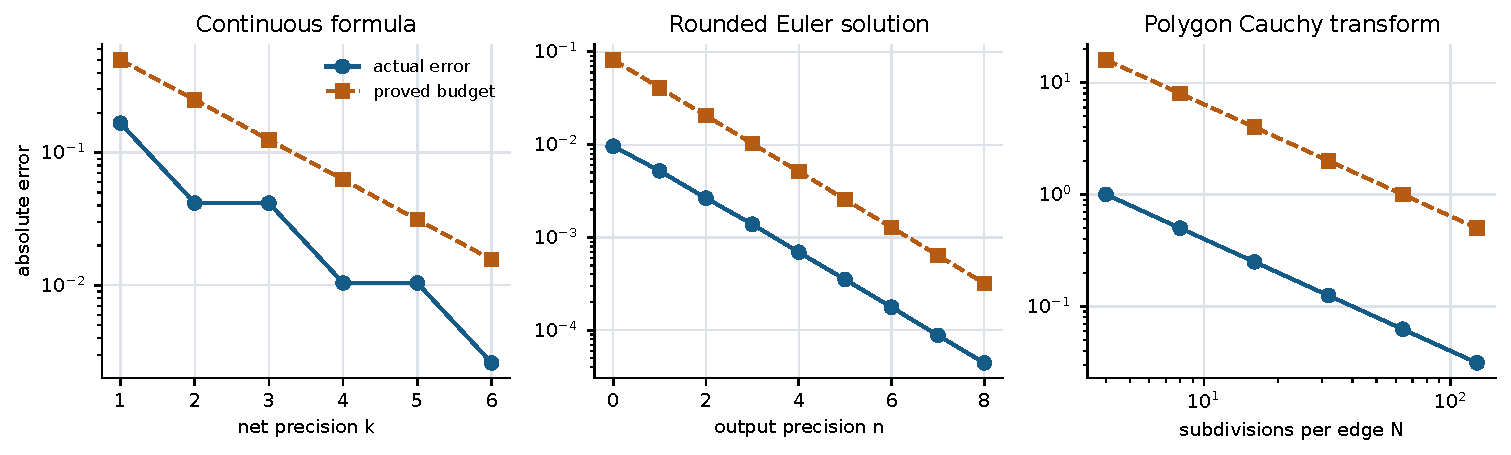
\includegraphics[width=\linewidth]{figures/validation.pdf}
\caption{Exact-rational examples, plotted after converting their final values
to floating point. Bounds are deliberately conservative. The finite checks
support implementation consistency; the universal arguments are in the text.}
\end{figure}

Run \texttt{python3 code/validate.py} from the extracted archive to reproduce
the exact checks, and \texttt{python3 code/plot\_validation.py} to regenerate
the figure. Run \texttt{pdflatex} twice on
\texttt{continuous\_mathematics\_in\_ipra.tex} to rebuild the report. The
validation receipt records that Lean compilation was not run. The source
manifest fixes the upstream commit and identifies the reviewed interfaces;
the archive does not silently substitute a newer repository state.

\clearpage
\begin{thebibliography}{99}
\bibitem{repo-plan}
V. Reshetnikov and contributors, \emph{ProveIt: iPRA unification plan}.
Pinned commit \texttt{5f3be02388442f16487d2dc5c2529961dd783d2b}.
\href{https://github.com/VladimirReshetnikov/ProveIt/blob/5f3be02388442f16487d2dc5c2529961dd783d2b/Logic/PrimitiveRecursiveArithmetic/UNIFICATION-PLAN.md}{Logic/PrimitiveRecursiveArithmetic/UNIFICATION-PLAN.md}.
All repository entries below use the same revision, inspected 20 November 2026.

\bibitem{repo-pr}
ProveIt, \emph{Intuitionistic primitive recursive arithmetic and natural deduction}.
\href{https://github.com/VladimirReshetnikov/ProveIt/blob/5f3be02388442f16487d2dc5c2529961dd783d2b/Logic/PrimitiveRecursiveArithmetic/ConciseIPRA/Lean/ConciseIPRA/PR.lean}{ConciseIPRA/PR.lean};
\href{https://github.com/VladimirReshetnikov/ProveIt/blob/5f3be02388442f16487d2dc5c2529961dd783d2b/Logic/PrimitiveRecursiveArithmetic/ConciseIPRA/Lean/ConciseIPRA/Deduction.lean}{ConciseIPRA/Deduction.lean}.

\bibitem{repo-setoid}
ProveIt, \emph{Interpretation through numerical presentations}.
\href{https://github.com/VladimirReshetnikov/ProveIt/blob/5f3be02388442f16487d2dc5c2529961dd783d2b/Logic/PrimitiveRecursiveArithmetic/Derivations/Lean/IPRADerivations/Foundations/SetoidInterpretation.lean}{Foundations/SetoidInterpretation.lean}.

\bibitem{repo-evaluator}
ProveIt, \emph{Universal evaluator obstruction}.
\href{https://github.com/VladimirReshetnikov/ProveIt/blob/5f3be02388442f16487d2dc5c2529961dd783d2b/Logic/PrimitiveRecursiveArithmetic/Derivations/Lean/IPRADerivations/Foundations/UniversalEvaluatorObstruction.lean}{Foundations/UniversalEvaluatorObstruction.lean}.

\bibitem{repo-finite-query}
ProveIt, \emph{Finite query demand and finite query tables}.
\href{https://github.com/VladimirReshetnikov/ProveIt/blob/5f3be02388442f16487d2dc5c2529961dd783d2b/Logic/PrimitiveRecursiveArithmetic/Derivations/Lean/IPRADerivations/Foundations/FiniteQueryDemand.lean}{Foundations/FiniteQueryDemand.lean};
\href{https://github.com/VladimirReshetnikov/ProveIt/blob/5f3be02388442f16487d2dc5c2529961dd783d2b/Logic/PrimitiveRecursiveArithmetic/Derivations/Lean/IPRADerivations/Foundations/FiniteQueryTable.lean}{Foundations/FiniteQueryTable.lean}.

\bibitem{repo-presented}
ProveIt, \emph{Presented categories}.
\href{https://github.com/VladimirReshetnikov/ProveIt/blob/5f3be02388442f16487d2dc5c2529961dd783d2b/Logic/PrimitiveRecursiveArithmetic/Derivations/Lean/IPRADerivations/Foundations/PresentedCategory.lean}{Foundations/PresentedCategory.lean}.

\bibitem{repo-yoneda}
ProveIt, \emph{Presentation-wise Yoneda}.
\href{https://github.com/VladimirReshetnikov/ProveIt/blob/5f3be02388442f16487d2dc5c2529961dd783d2b/Logic/PrimitiveRecursiveArithmetic/Derivations/Lean/IPRADerivations/Foundations/Yoneda.lean}{Foundations/Yoneda.lean}.

\bibitem{repo-gluing}
ProveIt, \emph{Uniform finite gluing}.
\href{https://github.com/VladimirReshetnikov/ProveIt/blob/5f3be02388442f16487d2dc5c2529961dd783d2b/Logic/PrimitiveRecursiveArithmetic/Derivations/Lean/IPRADerivations/Foundations/FiniteGluing.lean}{Foundations/FiniteGluing.lean}.

\bibitem{repo-guard}
ProveIt, \emph{Guarded totalization and overlapping branches}.
\href{https://github.com/VladimirReshetnikov/ProveIt/blob/5f3be02388442f16487d2dc5c2529961dd783d2b/Logic/PrimitiveRecursiveArithmetic/Derivations/Lean/IPRADerivations/Foundations/GuardedTotalization.lean}{Foundations/GuardedTotalization.lean};
\href{https://github.com/VladimirReshetnikov/ProveIt/blob/5f3be02388442f16487d2dc5c2529961dd783d2b/Logic/PrimitiveRecursiveArithmetic/Derivations/Lean/IPRADerivations/Foundations/OverlapBranches.lean}{Foundations/OverlapBranches.lean}.

\bibitem{repo-gronwall}
ProveIt, \emph{Discrete Gronwall}.
\href{https://github.com/VladimirReshetnikov/ProveIt/blob/5f3be02388442f16487d2dc5c2529961dd783d2b/Logic/PrimitiveRecursiveArithmetic/Derivations/Lean/IPRADerivations/Foundations/DiscreteGronwall.lean}{Foundations/DiscreteGronwall.lean}.

\bibitem{repo-ode-refinement}
ProveIt, \emph{ODE refinement}.
\href{https://github.com/VladimirReshetnikov/ProveIt/blob/5f3be02388442f16487d2dc5c2529961dd783d2b/Logic/PrimitiveRecursiveArithmetic/Derivations/Lean/IPRADerivations/Foundations/OdeRefinement.lean}{Foundations/OdeRefinement.lean}.

\bibitem{repo-ode-uniqueness}
ProveIt, \emph{ODE uniqueness}.
\href{https://github.com/VladimirReshetnikov/ProveIt/blob/5f3be02388442f16487d2dc5c2529961dd783d2b/Logic/PrimitiveRecursiveArithmetic/Derivations/Lean/IPRADerivations/Foundations/OdeUniqueness.lean}{Foundations/OdeUniqueness.lean}.

\bibitem{repo-ode-certificates}
ProveIt, \emph{ODE certificates: algebraic identities}.
\href{https://github.com/VladimirReshetnikov/ProveIt/blob/5f3be02388442f16487d2dc5c2529961dd783d2b/Logic/PrimitiveRecursiveArithmetic/Derivations/Lean/IPRADerivations/Analysis/OdeCertificates.lean}{Analysis/OdeCertificates.lean}.

\bibitem{oconnor2007}
R. O'Connor, \emph{A monadic, functional implementation of real numbers},
Mathematical Structures in Computer Science \textbf{17} (2007), 129--159.
\href{https://doi.org/10.1017/S0960129506005871}{doi:10.1017/S0960129506005871}.
\href{https://arxiv.org/abs/cs/0605058}{Author preprint, arXiv:cs/0605058}.
Used for context on constructive completion; the budgets in this report are
proved directly.

\bibitem{metric-model-theory}
I. Ben Yaacov, A. Berenstein, C. W. Henson and A. Usvyatsov,
\emph{Model theory for metric structures}, in Model Theory with Applications
to Algebra and Analysis, Volume 2, Cambridge University Press (2008), 315--427.
\href{https://math.univ-lyon1.fr/~begnac/articles/mtfms.pdf}{Author-hosted manuscript}.
The use of continuous truth values and infimum/supremum quantifiers is standard;
the finite-net bounds here are established independently.

\bibitem{kohlenbach-oliva}
U. Kohlenbach and P. Oliva, \emph{Proof mining: a systematic way of analysing
proofs in mathematics}, Proceedings of the Steklov Institute of Mathematics
\textbf{242} (2003), 136--164.
\href{https://www.eecs.qmul.ac.uk/~pbo/papers/paper004.pdf}{Author-hosted manuscript}.

\bibitem{avigad-feferman}
J. Avigad and S. Feferman, \emph{G\"odel's functional (Dialectica)
interpretation}, in Handbook of Proof Theory, S. R. Buss (ed.), Elsevier
(1998), 337--405.
\href{https://math.stanford.edu/~feferman/papers/dialectica.pdf}{Author-hosted draft}.
Used to distinguish higher-type functional interpretations from the
first-order proof target adopted here.
\end{thebibliography}

\end{document}
